\documentclass[letterpaper, 11pt]{IEEEtran}      % Use this line for a4 paper

%LatexiDiff ignore tikz:
% $: latexdiff -c "PICTUREENV=(?:picture|tikzpicture|DIFnomarkup)[\w\d*@]*" old.tex new.tex > diff.tex

%\IEEEoverridecommandlockouts                              %

%\usepackage{mathcomSTEP}

%\overrideIEEEmargins 
%\IEEEoverridecommandlockouts                              % This command is only needed if 
% you want to use the \thanks command

%\overrideIEEEmargins                                      % Needed to meet printer requirements.

% See the \addtolength command later in the file to balance the column lengths
% on the last page of the document

\onecolumn

\usepackage{mathptmx} 
\usepackage{times} 
\usepackage{amsmath} 
\usepackage{amsbsy} 
\usepackage{amssymb}

%\usepackage{newtxtext, newtxmath}
\usepackage{mathrsfs}
\usepackage{comment}
\usepackage[export]{adjustbox}
\usepackage{tikz}
\usetikzlibrary{external,positioning,decorations.pathreplacing,shapes,arrows,patterns}


\usepackage[hidelinks]{hyperref}
%\tikzexternalize[mode=list and make]
\usepackage{algorithmicx}
\usepackage{pgfplots}
\usepackage{graphicx}
\usepackage{pstool}
\usepackage[latin1]{inputenc}
\usetikzlibrary{arrows,shapes}
\usepackage{xifthen}
\usepackage{epic}
%\usepackage{caption}
\usepackage{epstopdf}

\newtheorem{thm}{\bf{Theorem}}
\newtheorem{cor}[thm]{\bf {Corollary}}
\newtheorem{lem}[thm]{\bf {Lemma}}
\newtheorem{prop}[thm]{\bf {Proposition}}
\newtheorem{example}{\bf {Example}}
\newtheorem{definition}{\bf {Definition}}
\newtheorem{rem}{\bf {Remark}}
\newtheorem{assump}{\bf {Assumptions}}

\newcommand{\ex}[1]{\ensuremath{\mathbb{E}\left[ #1\right]}}

\newcommand{\Var}[1]{\ensuremath{\mathrm{Var} \left[ #1\right]}}

\newcommand{\unif}{\mathsf{unif}}
\newcommand{\card}{\mathrm{card}}
\newcommand{\ARE}{\mathsf{ARE}}
\newcommand{\supp}{\mathrm{supp} }
\renewcommand\vec[1]{\ensuremath\boldsymbol{#1}}
\newenvironment{proof}{\paragraph*{Proof}}{\hfill$\square$ \newline}
\newcommand{\sgn}{\mathrm{sgn} }
\newcommand{\Prob}{\mathbb{P} }
\newcommand{\argmax}{\mathrm{argmax}}
\newcommand*{\QEDA}{\hfill\ensuremath{\square}}
\newcommand{\CEO}{\mathsf{CEO}}
\newcommand{\Ncal}{\mathcal{N}}

\newcommand{\enc}{\mathsf{enc}}
\newcommand{\est}{\mathsf{est}}

\tikzstyle{int}=[draw, fill=blue!10, minimum height = 1cm, minimum width=1.5cm,thick ]
\tikzstyle{sint}=[draw, fill=blue!10, minimum height = 0.5cm, minimum width=0.8cm,thick ]
\tikzstyle{sum}=[circle, fill=blue!10, draw=black,line width=1pt,minimum size = 0.5cm, thick ]
\tikzstyle{ssum}=[circle, fill=blue!10,draw=black,line width=1pt,minimum size = 0.1cm]
\tikzstyle{int1}=[draw, fill=blue!10, minimum height = 0.5cm, minimum width=0.7cm,thick ]
\tikzstyle{enc}=[draw, fill=blue!10, minimum height = 2.7cm, minimum width=1cm,thick ]
\tikzstyle{int}=[draw, fill=blue!10, minimum height = 1cm, minimum width=1.5cm,thick ]


\author{
    \IEEEauthorblockN{
Alon Kipnis\IEEEauthorrefmark{1} and   
    John C. Duchi\IEEEauthorrefmark{1}\IEEEauthorrefmark{2}  \\}
    \IEEEauthorblockA{\IEEEauthorrefmark{1}Stanford University, Department of Statistics \\}
    \IEEEauthorblockA{\IEEEauthorrefmark{2}Stanford University, Department of Electrical Engineering. }
}

\title{\LARGE \bf Mean Estimation from One-Bit Measurements}


\begin{document}
\graphicspath{{./Figs/}}
\maketitle
\thispagestyle{empty}
\pagestyle{empty}

%%%%%%%%%%%%%%%%%%%%%%%%%%%%%%%%%%%%%%%%%%%%%%%%%%%%%%%%%%%%%%%%%%%%%%%%%%%%%%%%
\begin{abstract}
We consider the problem of estimating the mean of a symmetric log-concave distribution under the following constraint: only a single bit per sample from this distribution is available to the estimator. We study the mean squared error risk in this estimation as a function of the number of samples, and hence the number of bits, from this distribution. 
%
Under an adaptive setting in which each bit is a function of the current sample and previously recorded bits, we show that the optimal relative efficiency compared to the sample mean is the efficiency of the median. %For example, in estimating the mean of a normal distribution, a constraint of one bit per sample incurs a penalty of $\pi/2$ in sample size compared to the unconstrained case. 
%
We also consider a distributed setting where each bit is only a function of a single sample. We show that the optimal efficiency of the adaptive setting can be attained by splitting the sample into two parts and allowing only a single adaptation. Otherwise, we show that no one sample estimation procedure can attain the optimal efficiency uniformly over all points in the parameter space.
%
%Finally, we analyze a distributed setting where the bits are obtained by comparing each sample against a prescribed threshold. Consequently, we consider the threshold density that minimizes the maximal MSE. 
%
Our results indicate that estimating the mean from one-bit measurements is equivalent to estimating the sample median from these measurements. In the adaptive case, this estimate can be done with vanishing error for any point in the parameter space. In the distributed case, this estimate can be done with vanishing error only for a finite number of possible values for the unknown mean. 
\end{abstract}

%{\color{red}  See LASSO results in http://arxiv.org/abs/1506.02181v1}


%%%%%%%%%%%%%%%%%%%%%%%%%%%%%%%%%%%%%%%%%%%%%%%%%%%%%%%%%%%%%%%%%%%%%%%%%%%%%%%%
\section{Introduction}
\label{sec:Intro}
Estimating parameters from data collected and processed by multiple units may be limited due to communication constraints between these units. 
%
For example, this scenario arises in sensor arrays where information is collected at multiple physical locations and transmitted to a central estimation unit. In these situations, the ability to estimate a particular parameter from the data is dictated not only by the quality of observations and their number but also by the available bandwidth for communicating between the sensors and the central estimator. The question that we ask is to what extent a parametric estimation task is affected by this constraint on communication, and what are the fundamental performance limits in estimating a parameter subject to such restriction. \par
%%
\begin{figure*}
\begin{center}
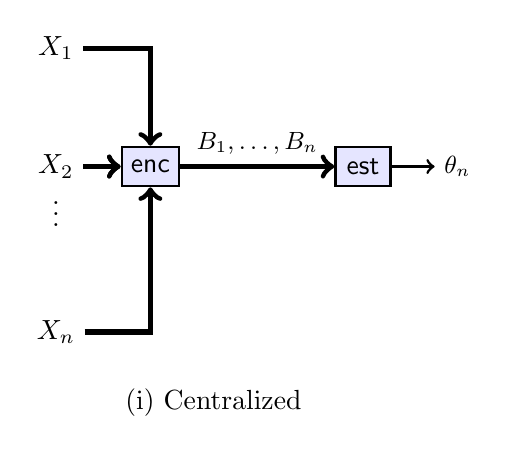
\begin{tikzpicture}[node distance=2cm,auto]

  \node at (0,0) (source) {$X_1$} ;
 \node[below of = source, node distance = 1.5cm] (source2) {$X_2$};
\node[below of = source2, node distance = 2.1cm] (source3) {$X_n$};

\node[int1, right of = source2, node distance = 1.2cm] (enc2) {$\enc$};  

\draw[->,line width = 2pt] (source2) -- (enc2); 
\draw[->,line width = 2pt] (source) -| (enc2); 
\draw[->,line width = 2pt] (source3) -| (enc2); 

\node[below of = source2, node distance = 0.5cm] {$\vdots$};

\draw[->,line width = 2pt] (source2) -- (enc2); 
\node[int1, right of = enc2, node distance = 2.7cm ] (est) {$\est$};

\draw[->,line width = 2pt] (enc2) -- node[above, xshift = 0cm] (mes2) {\small $B_1,\ldots,B_n$} (est);   

\node[right of = est, node distance = 1.2cm] (dest) {\small ${\theta}_n$};
%         \node [int1] (dec) [right of=dest, node distance = 1.5cm,  align=center] {\small Dec };
%\node [int1] (enc) [right of = dec, node distance = 3cm]{Enc}; 
%\draw[->,line width=2pt] (dec) -- (dest);
\draw[->, line width=1pt] (est) -- (dest);
\node at (2,-4.5) {(i) Centralized};
\end{tikzpicture}
%
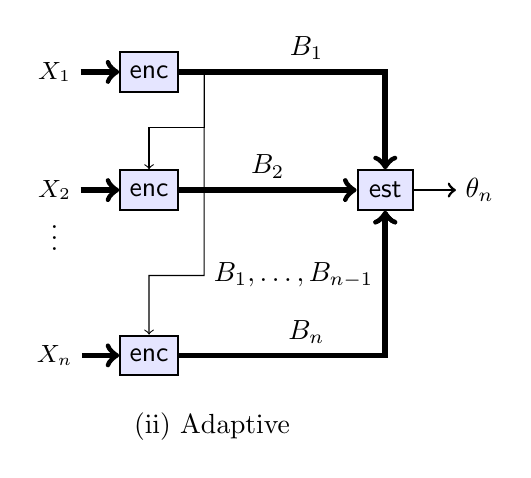
\begin{tikzpicture}[node distance=2cm,auto]
  \node at (0,0) (source) {\small $X_1$} ;
  \node[int1, right of = source, node distance = 1.2cm] (enc1) {$\enc$};  
\draw[->,line width = 2pt] (source) -- (enc1); 

 \node[below of = source, node distance = 1.5cm] (source2) {\small $X_2$};
\node[int1, right of = source2, node distance = 1.2cm] (enc2) {$\enc$};  
\draw[->,line width = 2pt] (source2) -- (enc2); 

\node[below of = source2, node distance = 2.1cm] (source3) {\small $X_n$};
\node[int1, right of = source3, node distance = 1.2cm] (enc3) {$\enc$};  
\draw[->,line width = 2pt] (source3) -- (enc3); 

\node[below of = source2, node distance = 0.5cm] {$\vdots$};
%\node[above of = source3, node distance = 1cm] (dist) {$X_i \sim P_X$};

\node[int1, right of = enc2, node distance = 3cm ] (est) {$\est$};
\draw[->,line width = 2pt] (enc1) -| node[above, xshift = -1cm] (mes1) {$B_1$} (est);   
\draw[->,line width = 2pt] (enc2) -- node[above, xshift = 0cm] (mes2) {$B_2$} (est);   

\draw[->] (enc1)+(0.7,0) -- +(0.7,-0.7) -| (enc2);

%\draw[dashed,->] (enc2)+(0.7,0) -- +(0.7,-0.7) -| +(0,-1.2);
\draw[->,line width = 2pt] (enc3) -| (est);   

%\node[below of = mes2, node distance = 1.5cm] (mes3) {$B_1,\ldots,B_{n-1} $};

\draw[->,line width = 2pt] (enc3) -| node[above, xshift = -1cm]  {$B_n$} (est);   

%\draw[->] (mes3.west) -- +(0,-0.5) -| (enc3);

\node[below right = 2.3cm and 0.7cm of 
enc1.center, yshift = 0.cm] (end) {$B_1,\ldots,B_{n-1}$};

\draw[->] (enc1)+(0.7,0) -- (end.west) -| (enc3);

\node[right of = est, node distance = 1.2cm] (dest) {${\theta}_n$};
%         \node [int1] (dec) [right of=dest, node distance = 1.5cm,  align=center] {\small Dec };
%\node [int1] (enc) [right of = dec, node distance = 3cm]{Enc}; 
%\draw[->,line width=2pt] (dec) -- (dest);
\draw[->, line width=1pt] (est) -- (dest);
\node at (2,-4.5) {(ii) Adaptive};
\end{tikzpicture}
%
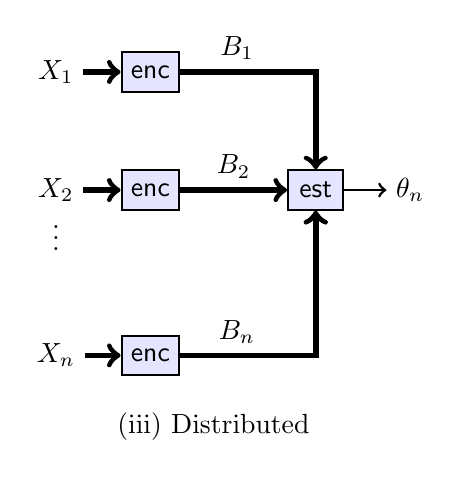
\begin{tikzpicture}[node distance=2cm,auto]
  \node at (0,0) (source) {$X_1$} ;
  \node[int1, right of = source, node distance = 1.2cm] (enc1) {$\enc$};  
\draw[->,line width = 2pt] (source) -- (enc1); 

 \node[below of = source, node distance = 1.5cm] (source2) {$X_2$};
\node[int1, right of = source2, node distance = 1.2cm] (enc2) {$\enc$};  
\draw[->,line width = 2pt] (source2) -- (enc2); 

\node[below of = source2, node distance = 2.1cm] (source3) {$X_n$};
\node[int1, right of = source3, node distance = 1.2cm] (enc3) {$\enc$};  
\draw[->,line width = 2pt] (source3) -- (enc3); 

%\node[above of = source3, node distance = 1cm] (dist) {$X_i \sim {\Ncal} \left(\theta, \sigma^2 \right)$};
\node[below of = source2, node distance = 0.5cm] {$\vdots$};

\node[int1, right of = enc2, node distance = 2.1cm ] (est) {$\est$};
\draw[->,line width = 2pt] (enc1) -| node[above, xshift = -1cm] (mes1) {$B_1$} (est);   

\draw[->,line width = 2pt] (enc2) -- node[above, xshift = 0cm] (mes2) {$B_2$} (est);   

\draw[->,line width = 2pt] (enc3) -| (est);   

\draw[->,line width = 2pt] (enc3) -| node[above, xshift = -1cm]  {$B_n$} (est);   

\node[right of = est, node distance = 1.2cm] (dest) {${\theta}_n$};
%         \node [int1] (dec) [right of=dest, node distance = 1.5cm,  align=center] {\small Dec };
%\node [int1] (enc) [right of = dec, node distance = 3cm]{Enc}; 
%\draw[->,line width=2pt] (dec) -- (dest);
\draw[->, line width=1pt] (est) -- (dest);
\node at (2,-4.5) {(iii) Distributed};
\end{tikzpicture}
\end{center}
\caption{\label{fig:setup} 
Three encoding settings: (i) Centralized  -- an encoder sends $n$ bits after observing $n$ samples. (ii) Adaptive (sequential) --  the $i$th encoder sends the bit $B_i$ depending on its private sample $X_i$ and previous bits $B_1,\ldots,B_{i-1}$. (iii) Distributed  -- each encoder send the bit $B_i$ based on its private sample $X_i$ only.}
\end{figure*}
%%

This paper answers this question in a particular setting: the estimation of the mean $\theta$ of a symmetric log-concave distribution with finite variance, under the constraint that only a single bit can be communicated on each sample from this distribution. As it turns out, the ability to share information before committing on each one-bit message dramatically affects the performance in estimating $\theta$. We, therefore, distinguish among the three settings illustrated in Figure~\ref{fig:setup}
\begin{itemize}
 \item[(i)\,\,] \emph{Centralized} encoding: all $n$ encoders confer and produce a single message consists of $n$ bits.
 \item[(ii)\,] \emph{Adaptive} or \emph{sequential} encoding: The $n$th encoder observes the $n$th sample and the $n-1$ previous bits.
 \item[(iii)] \emph{Distributed} encoding: The $n$th message is only a function of the $n$th sample.
 \end{itemize}
Evidently, as far as information sharing is concerned, settings (iii) is a more restrictive version of (ii) which is more restrictive than (i). Below are three application examples for each of the settings (i)-(iii) above, respectively:
\begin{itemize}
\item {\bf Signal acquisition:} A quantity is measured $n$ times at different instances. The results are averaged in order to reduce measurement noise and the averaged result is then stored or communicated using $n$ bits. 
\item {\bf Analog-to-digital conversion:} A sigma-delta modulator (SDM) converts an analog signal into a sequence of bits by sampling the signal at a very high rate and then using one-bit threshold detector combined with a feedback loop to update an accumulated error state \cite{1092194}. Therefore, the expected error in tracking an analog signal using an SDM falls under our setting (ii) when we assume that the signal at the input to the modulator is a constant (direct current) corrupted by, say, thermal noise \cite{53738}. Since the sampling rates in SDM are usually many times more than the bandwidth of its input, analyzing SDM under a constant input provides meaningful lower bound even for non-constant signals.
\item {\bf Privacy:} A business entity is interested in estimating the average income of its clients. In order to keep this information as confidential as possible, each client independently provides an answer to a yes/no question related to its income.
\end{itemize}
%
We measure the performance in estimating $\theta$ by the quadratic risk. For an estimator with finite quadratic risk $R_n$, we are interested in particular in the limit
\begin{equation}
\label{eq:ARE_def}
\lim_{n\to \infty} \frac{\sigma^2/n}{R_n},
\end{equation}
describing the \emph{asymptotic relative efficiency} (ARE) of this estimator compared to an estimator whose variance decreases as $\sigma^2/n+o(n^{-1})$. Estimators of this form include the empirical mean of the samples, and, under some conditions, the optimal Bayes estimator. \par
%
In addition to the examples above, the excess risk in estimating a fixed parameter due to a one-bit per sample constraint is useful in bounding from below the excess risk in estimating signals from thier noisy one-bit quanitzed noisy measurements. Specifically, the excess risk or ARE we derive serve as the most optimistic estimate for the risk in estimating under one-bit per measurement constraint signals changing over time or space. Such estimation settings are considered in \cite{baraniuk2017exponential, jacques2013robust, plan2013one, li2017channel, choi2016near}. \par

% given a prior distribution on the space $\Theta$ where $\theta$ resides. \\

In setting (i), the estimator can evaluate the optimal mean estimator (e.g., the sample mean in the Gaussian case) and then quantize it using $n$ bits. Since the accuracy in describing the empirical mean decreases exponentially in $n$, the error due to quantization is negligible compared to the quadratic risk in estimating the mean \cite{720540}. Therefore, the ARE in this setting is $1$. Namely, asymptotically, there is no loss in performance due to the communication constraint under centralized encoding. 
%
In this paper we show that a similar result does not hold in setting (ii): the ARE of any adaptive estimation scheme is at most the ARE of the sample median. Specifically, when the samples are drawn from the normal distribution, this ARE equals $2/\pi$, showing that the one-bit constraint increases the effective sample size in estimating $\theta$ by at least $\pi/2$ compared to estimating it without the bit constraint. We also show that this lower bound on the ARE is tight by providing an estimator that attains it. In fact, we show that only one adaptiveness, as illustrated in Figure~\ref{fig:one_round} is enough to achieve the optimal ARE. 
%
Clearly, the penalty on the sample size in setting (iii) is at least as large as that in setting (ii). We show, however, that unlike in setting (ii), there is no distributed estimation scheme that is uniformly optimal in the sense that it attains the ARE of the sample median for all $\theta$ in the parameter space. This result is obtained by establishing local asymptotic normality of regularly enough encoding procedures for setting (iii), resulting in an exact characterization of the ARE of such procedures. To summarize our contributions, we establish that the optimal ARE in settings (i) is $1$, the optimal ARE in setting (ii) is ARE of the sample median, and no uniformly optimal procedure exists in setting (iii). 

% Instead, in setting (iii) we restrict ourselves to estimators from messages obtained by comparison against a prescribed value (that may be different for each sample). We show that the maximum likelihood (ML) estimator for $\theta$ from these messages is asymptotically local minimax, and its asymptotic variance is strictly greater than the variance of the median. Thus, at least when limited to threshold detection, the ability to adapt the threshold allows for a more efficient estimation. %This is in contrast to the \\ counterpart of our setting where $\theta$ is taken from a finite space 

It is important to note that although the ARE in setting (i) is one, this scheme already poses a non-trivial challenge for the design and analysis of optimal encoding and estimation procedures. Indeed, representing an unknown random quantity using $n$ bits is equivalent to designing a $2^n$ levels scalar quantizer \cite{gray1998quantization}. However, the optimal design of this quantizer depends on the distribution of its input, which is the goal of our estimation problem and hence its exact value is unknown. As a result, a non-trivial exploration-exploitation trade-off arises even in setting (i). 
%Note that the only missing parameter in our setting is the mean, which, under setting (i), is known to the encoder with uncertainty interval proportional to $\sigma/\sqrt{n}$. 
Therefore, while uncertainty due to quantization decreases exponentially in the number of bits $n$, hence the ARE is $1$, it is still difficult to derive an exact expression for the MSE in this setting. 
%
The situation is even more involved in the adaptive encoding setting (ii): an encoding and estimation strategy that is optimal for $n-1$ adaptive one-bit messages of a sample of size $n-1$ may not lead to a globally optimal strategy upon the recipient of the $n$th sample. Conversely, any one-step optimal strategy, in the sense that it finds the best one-bit message as a function of the current sample and the previous $n-1$ messages, is not guaranteed to be globally optimal. Therefore, while we characterize the optimal one-bit message given the previous messages, this characterization does not necessarily lead to an upper bound on the ARE. Instead, our result on the maximal ARE is obtained by bounding the Fisher information of any $n$ adaptive messages and using an appropriate information inequality. \par
%
%In addition to encoding and estimation schemes that lead to optimal results, we also consider two additional ``natural'' schemes. Specifically, in setting (ii) we consider the one-bit optimal scheme, i.e., the case of a greedy encoder that given the $n$th sample and the previous $n-1$ bits, provides a bit that minimizes the $n$-step MSE. In setting (iii) we also consider the case where the messages are obtained by comparing each sample against a prescribed threshold. This threshold may be different across samples and is assumed deterministic (independent of the data). 


\subsection*{Related Works}
When the variance $\sigma^2$ is negligible compared the to desired accuracy, the task of finding $\theta$ using one-bit queries in the adaptive setting (ii) is solved by a bisection style method over the parameter space. Therefore, the general case of non-zero variance is reminiscent of the noisy binary search problem with a possibly infinite number of unreliable tests \cite{cicalese2002least, Karp:2007:NBS:1283383.1283478}. However, since we assume a continuous parameter space, a more closely related problem is that of one-bit analog-to-digital conversion of a constant input corrupted by Gaussian noise. Using an SDM, Wong and Gray \cite{53738} showed that the output of the modulator converges to the true constant input almost surely, so that an SDM provides a consistent estimator for setting (ii). The rate of this convergence, however, was not analyzed and cannot be derived from the results of \cite{53738}. In particular, our results for setting (ii) imply that the asymptotic rate of convergence of the MSE in SDM to a constant input under an additive white Gaussian noise is at most $\sigma^2\pi/2$ over the number of feedback iterations. Baraniuk et. al \cite{baraniuk2017exponential} also considered adaptive one-bit measurements in the context of analog-to-digital conversion, although without noise at the input. By establishing the lower bound of $\sigma^2\pi/2n$ on the MSE, we show that the main results of \cite{baraniuk2017exponential}, an exponential MSE decaying rate, does not hold in the noisy setting. Stated otherwise, the MSE in the setting of \cite{baraniuk2017exponential} may decay exponentially up to the noise level, after which it decays at most as $\sigma^2\pi/2n$. \par
%
One-bit measurements in the distributed setting (iii) was considered in \cite{904560,4244748, 6882252, chen2010performance, 5184907}, but without optimizing the encoders and their detection rules. Consequently, the performance derived in these works are not optimal. 
 % analyzed the estimation from distributed quantized measurements when the same detection rule is applied by all encoders. However, the error criterion considered in these works is the Fisher information rather than the MSE risk or ARE criterion. \par
%Once the decision rule of each encoder is fixed, the optimal estimation of $\theta$ is determined using the maximum a posteriori probability rule. Hence, the distributed setting is reduced to finding the optimal decision rule of each encoder.
The work of \cite{52470} addresses the counterpart of our setting (iii) in the case of hypothesis testing, although the results there cannot be extended to parametric estimation. When the parameter space $\Theta$ is finite, Tsitsiklist \cite{tsitsiklis1988decentralized} showed that when the cardinality of $\Theta$ is at most $M$ and the probability of error criterion is used, then no more than $M(M-1)/2$ different detection rules are necessary in order to attain probability of error decreasing exponentially with the optimal exponent. %That is, beyond $M(M-1)/2$ some decision rules can be repeated without losing optimality.
Furthermore, in a version of this problem for the adaptive setting \cite{5751320}, it was shown that, with specific two-stage feedback, there is no gain in feedback compared to the fully distributed setting. Our results imply that the ARE in the distributed setting with threshold detection rules is strictly larger than that in the adaptive setting for almost all points in $\Theta$, suggesting that the case where the cardinality of $\Theta$ is finite is different from the case where $\Theta$ is an open set.\par
%
As we explain in detail in Section~ \ref{sec:preliminary}, the remote multiterminal source coding problem, also known as the CEO problem \cite{berger1996ceo, viswanathan1997quadratic, oohama1998rate, prabhakaran2004rate}, leads to lower bounds on the MSE in setting (iii). For the case of a Gaussian distribution, this lower bound bounds the ARE to be at most $3/4$. Thus, while this bound on the ARE provides no new information compared to the upper bound of $2/\pi$ we derive for setting (ii), it shows that the distributed nature of the problem is not a limiting factor in achieving MSE close to optimum even under the one bit per sample constraint. 
 \par
% 
Finally, we note that minimax estimation under limited communication with an arbitrary number of bits per node was considered in 
\cite{zhang2013information, duchi2014optimality}. The specialization of the results in \cite{zhang2013information, duchi2014optimality} to our settings (ii) and (iii) leads to looser lower bounds then the ones we derive in this paper. Looser bounds can also be obtained from works considering general inference and distributed estimation problems under data compression constraint \cite{DBLP:journals/corr/abs-1802-08417, zhang1988estimation, han2018distributed, xu2017information, Barnes2018}. In particular, the subsequent work of \cite{Barnes2018} uses an approach similar to ours to derive lower bound on the error in various parametric estimation problems from quantized measurements. \par


The remainder of this paper is organized as follows. In Section~\ref{sec:problem} we describe the problem and useful notation. In Section~\ref{sec:preliminary} we provide two simple bounds on the efficiency and MSE. Our main results for the adaptive and distributed cases are given in Sections~\ref{sec:sequential} and \ref{sec:distributed}, respectively. In Section~\ref{sec:conclusions} we provide concluding remarks. 

\section{Problem Formulation \label{sec:problem}}

Let $f(x)$ be a symmetric and log-concave density function with a finite second moment $\sigma^2$. For $\theta \in \Theta$, denote by $P_X$ the probability distribution with density $f\left( x-\theta \right)$. Therefore, $P_X$ is an absolutely continuous log-concave distribution with mean $\theta$ and variance $\sigma^2$. Symmetry and log-concavity of $f(x)$ imply that $P_X$ is strongly unimodal (has a unique local maxima) with its mode at $x =\theta$ \cite{ibragimov1956composition}. We further assume that the \emph{parameter space} $\Theta$ is a closed interval of the real line. 
\par
In some situations it is useful to assume that $\theta$ is drawn once from the prior distribution $\pi$ on $\Theta$. In this case we assume that $\pi$ is an absolutely continuous distribution, and denote its density by $\pi(\theta)$, i.e., $\pi(d\theta) = \pi(\theta)d\theta$.  
\par
The random variables $X_1,\ldots,X_n$ represent $n$ independent samples from $P_X$. 
We are interested in estimating $\theta$ from a set of $n$ binary messages $B_1,\ldots,B_n$, obtained from $X_1,\ldots,X_n$ under three possible scenarios illustrated in Figure~\ref{fig:setup}: 
\begin{itemize}
\item[(i)~~] Centralized $B_i(X_1,\ldots,X_n)$, $i=1,\ldots,n$.
\item[(ii)~] Adaptive $B_i(X_i,B_1,\ldots,B_{i-1})$, $i=2,\ldots,n$.
\item[(iii)] Distributed $B_i(X_i)$, $i=1,\ldots,n$.
\end{itemize}

The performance of an estimator ${\theta}_n \triangleq {\theta}_n(B^n)$ in any of these cases is measured according to the quadratic risk:
\begin{equation}
\label{eq:error_def}
R_n \triangleq \mathbb E\left({\theta}_n - \theta \right)^2,
\end{equation}
where the expectation is taken with respect to the distribution of $X_1,\ldots,X_n$ and, whenever available, a prior distribution $\pi(\theta)$ over $\Theta$.  
%It is well known that minmax estimation error 
%\begin{equation}
%R_n = \min \sup_{\theta \in \Theta}  \mathbb E\left[ \left({\theta}_n - \theta \right)^2 | \theta \right],
%\end{equation}
%can be obtained from $R_n$ by assuming a particular least favorable prior distribution on the parameter space $\Theta$ \cite{casella1981}. 
%
The main problems we consider in this paper are the minimal value of \eqref{eq:error_def}, as a function of $n$ and $f(x)$, under different choices of the encoding functions in cases (i), (ii), and (iii). \par

We give particular attention to the ARE of estimators with respect to an asymptotically normal efficient estimator that is not subject to the bit constraint. Specifically, let $\{a_n,\,n\in \mathbb N\}$ be a sequence such that 
\[
\sqrt{a_n}\left({\theta}_n - \theta\right) \overset{d}{\longrightarrow} \Ncal(0, \sigma^2).
\]
Then the ARE of ${\theta}_n$ with respect to an unconstrained efficient estimator for $\theta$ is defined as \cite[Def. 6.6.6]{lehmann2006theory}
\[
\ARE({\theta}_n) \triangleq
\lim_{n\rightarrow \infty} \frac{a_n}{n}. 
\]
Note that in the special case where there exists $V \in \mathbb R$ such that
\[
a_n \mathbb E \left({\theta}_n - \theta \right)^2 = V + o(1),
\]
with $o(1)\to 0$ as $n\to \infty$, then the ARE of ${\theta}_n$ is finite and equals $\sigma^2/V$. \par

In addition to the notation above, we also denote by $F(x)$ the cumulative distribution function of $X_i$, and define
\begin{equation} \label{eq:eta_def}
\eta(x) \triangleq \frac{f^2(x)}{F(x)(1-F(x))} =  \frac{f(x)f(-x)}{F(x)F(-x)}, 
\end{equation}
where the last equality is due to symmetry of $f(x)$. We note that 
\begin{equation}
\label{eq:eta_h}
\eta(x) = h(x)h(-x) = f(x) \left( h(x) + h(-x) \right), 
\end{equation}
where 
\[
h(x) \triangleq \frac{f(x)}{1-F(x)} = \frac{f(x)}{F(-x)}
\]
is the \emph{hazard} function (a.k.a. \emph{failure rate} or \emph{force of mortality}), which is a monotone increasing function since $f(x)$ is log-concave \cite{bagnoli2005log}. 
%
For $f(x)$ the normal density, it is shown in \cite{Samford1953} and \cite{hammersley1950estimating} that $\eta(x)$ is a strictly decreasing function of $|x|$, as illustrated in Fig.~\ref{fig:eta}. 
%
In this paper we only consider the normal distribution and other log-concave symmetric distributions for which this property of $\eta(x)$ holds. Specifically, we require the following:
\begin{assump} \label{assump:failure_rate}
 $\eta(x)$ has a unique maximum (at the origin) and is a non-increasing function of $|x|$. 
\end{assump}
%That is, Assumption~\ref{assump:failure_rate} says that $\eta'(x) < 0 $ for all $x>0$. 
Under this assumption we have, 
\[
4f^2(x) \leq \eta(x) \leq \eta(0),
\] 
%
where $\eta(0) = 4 f^2(0)$ is the asymptotic variance of the sample median. Combined with log-concavity of $f(x)$, Assumption~\ref{assump:failure_rate} implies that $\eta(x)$ vanishes as $|x|\rightarrow \infty$. \par
%
Assumption~\ref{assump:failure_rate} is satisfied, for example, by the generalized normal distributions with a shape parameter between $1$ and $2$ (including normal and Laplace distributions). Symmetric log-concave distributions that do not satisfy Assumption~\ref{assump:failure_rate} include the uniform distribution and the generalized normal distribution with shape parameter greater than $2$.\par

\begin{figure}
\begin{center}
\begin{tikzpicture}[scale = 0.6]
\begin{axis}[
width=8cm, height=6cm,
xmin = -3, xmax=3, 
restrict y to domain = 0:100,
ymin = 0,
ymax = 0.9,
samples=10, 
xlabel= $x$,
xtick={-2,-1,0,1,2},
xticklabels={-2,-1,0,1,2},
ytick={0,0.3989423,0.6366198},
yticklabels={0,$\frac{1}{\sqrt{2 \pi}}$,$2/\pi$},
line width=1.0pt,
mark size=1.5pt,
ymajorgrids,
xmajorgrids,
legend style= {at={(1,1)},anchor=north east,draw=black,fill=white,align=left}
]
\addplot[color = blue, solid, smooth] plot table [x = x, y = y, col sep=comma] {./Figs/eta.csv};
\addlegendentry{$\eta(x)$};
\addplot[domain = -5:5, samples = 50, color = red, solid, smooth]  {exp(-x^2/2) / sqrt(2*3.14159)};
\addlegendentry{$\phi(x)$};
\addplot[domain = -5:5, samples = 50, color = black, solid, dashed]  {4*exp(-x^2) / (2*3.14159)};
\addlegendentry{$4\phi^2(x)$};

\end{axis}
\end{tikzpicture}
%
\begin{tikzpicture}[scale = 0.6]
\begin{axis}[
width=8cm, height=6cm,
xmin = -4, xmax=4, 
restrict y to domain = -10:0,
ymin = -10,
samples=10, 
xlabel= $x$,
xtick={-3,-2,-1,0,1,2,3},
xticklabels={-3,-2,-1,0,1,2,3},
ytick={0,-0.45158,-0.919},
yticklabels={0,,},
line width=1.0pt,
mark size=1.5pt,
ymajorgrids,
xmajorgrids,
legend style= {at={(1,1)},anchor=north east,draw=black,fill=white,align=left}
]
\addplot[color = blue, solid, smooth] plot table [x = x, y = logy, col sep=comma] {./Figs/eta.csv};
\addlegendentry{$\log \eta(x)$};
\addplot[domain = -5:5, samples = 30, color = red, solid, smooth]  {-(x)^2/2 -0.9189};
\addlegendentry{$\log \phi(x)$};
\end{axis}
\end{tikzpicture}
\caption{
The function $\eta(x) = f^2(x) / F(x)F(-x)$ for $f(x) = \phi(x)$ the standard normal density.
\label{fig:eta}
}
\end{center}
\end{figure}

\section{Consistent Estimation and Off-the-shelf Bounds \label{sec:preliminary}}
%
In this section we adapt known results to derive lower and upper bounds on the relative efficiency under setting (iii). These bounds establish the following facts:
\begin{itemize}
\item[I.] A consistent estimator with an asymptotically normal distribution always exists in setting (iii), and hence in setting (ii). 
\item[II.] For the normal distribution, the ARE in setting (iii) is at most $3/4$. Namely, under setting (iii), all estimators are strictly inferior compared to the sample mean. 
\end{itemize}

\subsection{Consistent Estimation}
Fix $\theta_0 \in \mathbb R$ and define the $i$th message by 
\[
B_i = \mathbf 1_{X_i>\theta_0}, 
\]
where $\mathbf 1_A$ is the indicator of the event $A$. We have
\[
P_n \triangleq\frac{1}{n} \sum_{i=1}^n B_i \overset{a.s.}{\rightarrow} F(\theta - \theta_0),  
\]
so that 
\begin{equation}
\label{eq:estimator_naive}
{\theta}_n = \theta_0 + F^{-1}\left( P_n \right)
\end{equation}
is a consistent estimator for $\theta$ in the distributed setting of Figure~\ref{fig:setup}-(iii), where we note that $F(x)$ is invertible over the support of $f(x)$ which is a connected set due to log-concavity. Furthermore, the variance of $P_n$ is $F(\theta-\theta_0)\left(1-F(\theta-\theta_0)\right)$, and hence the delta method implies that ${\theta}_n$ is asymptotically normal with variance 
\begin{equation} 
 \frac{F(\theta-\theta_0)\left(1-F(\theta-\theta_0)\right)}{f^2(\theta-\theta_0)} = \frac{1}{
\eta(\theta-\theta_0)}.
\end{equation}
In particular, the ARE of ${\theta}_n$ equals $\eta(\theta - \theta_0)\sigma^2$. In other words, for a prescribed accuracy, ${\theta}_n$ of  \eqref{eq:estimator_naive} estimates $\theta$ with sample size that is $\eta(\theta- \theta_0)  \sigma^2$ times the samples size required for the sample mean. \par
%
%
Assumption~\ref{assump:failure_rate} implies that for  all $n$ large enough the ARE of ${\theta}_n$ of \eqref{eq:estimator_naive} is never greater than $\eta(0)$, which is the ARE of the sample median. This ARE is attained only when $\theta_0 = \theta$, whereas $\theta$ is apriori unknown. Since $\eta(x)$ vanishes as $|x|\rightarrow \infty$, the ARE of ${\theta}_n$ may be very small when $\theta$ is away from $\theta_0$. As an example, when $f(x)$ is a normal density, the ARE of ${\theta}_n$ is less than $\approx 0.14$ when $\theta_0$ is $2$ standard deviations from $\theta$. Therefore, the estimator ${\theta}_n$ has little practical value unless the radius of $\Theta$ is small compared to the standard deviation. \par 
It is suggested that we can attain lower variance in estimation by updating the threshold value $\theta_0$ in \eqref{eq:estimator_naive} after observing one or a batch of the single bit messages. Schemes with such adaptation fall within the adaptive setting of Figure~\ref{fig:setup}-(ii) which we consider in Section~\ref{sec:sequential}. \par

\subsection{Multiterminal Source Coding \label{sec:ceo}}
The CEO setting considers the estimation of a sequence $\theta_1,\theta_2\ldots$, where a noisy version of each $\theta_i$ is available at $n$ terminals. At each terminal $i$, an encoder observes the $k$ noisy samples
\[
X_{i,j} = \theta_j + Z_{i,j},\qquad j=1,\ldots,k, \qquad i = 1,\ldots,n,
\]
and transmits $r_i k$ bits to a central estimator  \cite{berger1996ceo}. The central estimator produces an estimates ${\theta}_1,\ldots,{\theta}_k$ with the goal of minimizing the quadratic risk:
\[
R_{\CEO} = \frac{1}{k} \sum_{j=1}^k \mathbb E \left[\left(\theta_j - {\theta}_j \right)^2 \right]. 
\]
Note that any distributed encoding scheme using one-bit per sample can be replicated $k$ times and thus leads to a legitimate encoding and estimation scheme for the CEO problem with $r_1=\ldots=r_n = 1$. It follows that, assuming that $\theta$ is drawn once from the prior $\pi(d\theta)$, our mean estimation problem from one-bit samples under distributed encoding corresponds to the CEO setting with $k=1$ realization of $\theta$ observed under noise at $n$ different locations, and communicated at each location using an encoder sending a single bit. 
%
Consequently, a lower bound on the MSE in estimating $\theta$ in the distributed encoding setting is given by the minimal MSE in the CEO setting as $k \to \infty$. Note that the difference between the CEO setting and ours lays in the privilege of each of the encoders to describe $k$ realizations of $\theta$ using $k$ bits with MSE averaged over these realizations, rather than a single realization using a single bit in ours. 
 \par
When the prior on $\theta$ and the noise corrupting it at each location are Gaussian, the optimal encoding scheme and its asymptotic risk as $k$ goes to infinity were fully characterized in \cite{prabhakaran2004rate}. Furthermore, the work of \cite{chen2004upper} provided an expression for quadratic risk attained in the CEO setting under Gaussian priors. Adapting to our setting, this expression provides the following proposition:
\begin{prop} \label{prop:ceo_lower_bound}
Assume that $\Theta = \mathbb R$ and $\pi(\theta) = \Ncal(0,\sigma_\theta^2)$ where $\sigma_\theta^2 \in \mathbb R$ is arbitrary. Then any estimator ${\theta}_n$ of $\theta$ in the distributed setting satisfies
\begin{equation} \label{eq:ceo_bound}
 n\mathbb E \left( \theta - \theta_n \right)^2 \geq \frac{4}{3} \sigma^2 + O(n^{-1}),
\end{equation}
where the expectation is with respect to $\theta$ and $X^n$.
\end{prop}

\begin{proof}
See Appendix~\ref{app:proof:prop_ceo_lower_bound}.
\end{proof}

From the formulation of the CEO problem, it follows that the difference between the MSE lower bound \eqref{eq:ceo_bound} and the actual MSE in the distributed setting (case (iii)) is attributed to the ability to perform coding over blocks. Namely, each encoder in the CEO setting may encode an arbitrary number of $k$ independent realizations of $\theta$ using $k$ bits, versus only one realization with one bit in ours. In other words, it is the ability to exploit the geometry of a high-dimensional product probability space that distinguishes between the CEO problem with one bit per encoder on average and the mean estimation problem from one-bit measurements in the distributed setting. 

\section{Adaptive Estimation \label{sec:sequential}}
The first main results of this paper, as described in Theorem~\ref{thm:adpative_lower_bound} below, states that the ARE of any adaptive estimator cannot be larger than $\eta(0)\sigma^2$, which is the ARE of the median of the sample $X_1,\ldots,X_n$. We also provide a particular adaptive estimation scheme that attains this maximal efficiency. %Finally, in Theorem~\ref{thm:opt_one_step}, we provide an adaptive estimation scheme that is one-step optimal in the sense that at each step $i$, the chosen message $B_i$  minimizes the MSE given $X_i$ and the previous $i-1$ messages. %Numerical simulations for the case of $f(x)$ the normal density function shows that the ARE of the estimator described by this scheme is $\eta(0)\sigma^2$. 

\subsection{Limited efficiency in the adaptive setting}
Our first result asserts that the ARE of any adaptive encoding and estimation scheme is bounded from above by $\eta(0)\sigma^2$. %This result follows from the following theorem:
\begin{thm}[maximal relative effeciency] \label{thm:adpative_lower_bound}
Let ${\theta}_n$ be any estimator of $\theta$ in the adaptive setting of Figure~\ref{fig:setup}-(ii). Assumes that $\pi(\theta)$ converges to zero at the endpoints of the interval $\Theta$. Then
\[
n\mathbb E\left[ (\theta-{\theta}_n)^2 \right] \geq   \frac{n}{ 4f^2(0) n + I_0},
\]
where 
\[
I_0 = \mathbb E \left( \frac{d}{d\theta} \log \pi (\theta) \right)^2
\]
is the Fisher information with respect to a location model in $\theta$. 
\end{thm}

\subsubsection*{Proof}
%We first bound from above the Fisher information of any set of $n$ one-bit messages with respect to $\theta$. The result then follows using the van-Trees inequality which bounds from below the risk of any estimator of $\theta$ by the inverse of the expected value of the aforementioned Fisher information plus $I_0$. The details are in
See Appendix~\ref{proof:thm:adpative_lower_bound}.\par

Theorem~\ref{thm:adpative_lower_bound} implies that any estimator ${\theta}_n$ from any adaptive encoding scheme satisfies
\[
n\mathbb E\left[ (\theta-\theta_n)^2 \right] \leq  \frac{1}{4f^2(0)}+O(n^{-1}),
\]
and 
\[
\ARE({\theta}_n) \leq 4f^2(0)\sigma^2 = \eta(0)\sigma^2.
\]

Next, we present an adaptive encoding and estimation scheme that attains the maximal ARE of $\eta(0)\sigma^2$. 

\subsection{Asymptotically optimal estimator}
Let $\left\{ \gamma_n \right\}_{n\in \mathbb N}$ be a strictly positive sequence. Consider the following estimator ${\theta}_n$ for $\theta$:  
\begin{equation}
\label{eq:sgd_alg}
\theta_n = \theta_{n-1} +  \gamma_n B_n, \quad n = 1,2,\ldots,
\end{equation}
where 
\begin{equation}
B_n = B_n (X_n,\theta_{n-1}) =\sgn (X_n - \theta_{n-1}).
\end{equation}
Define the $n$th step estimation as
\begin{equation} \label{eq:sgd_est}
\bar{\theta}_n =  \frac{1}{n} \sum_{i=1}^n  \theta_i. 
\end{equation}

We have the following results:
\begin{thm} \label{thm:sgd}
Consider the sequence $\left\{\bar{\theta}_n \right\}_{n\in \mathbb N}$ defined by \eqref{eq:sgd_est}. 
\begin{enumerate}
\item[(i)] Assume that $\left\{ \gamma_n \right\}_{n\in \mathbb N}$ satisfies
\begin{equation} \label{eq:conditions1}
\begin{cases}
\frac{\gamma_n - \gamma_{n+1}}{\gamma_n} = o(\gamma_n), &  \\
\sum_{n=1}^\infty \frac{\gamma_n^{(1+\lambda)/2}} {\sqrt{n}} < \infty, & 
\mathrm{for~some~}0< \lambda \leq 1
\end{cases}
\end{equation}
(e.g., $\gamma_n = n^{-\beta}$ for $\beta \in (0,1)$). Then
\[
\sqrt{n}\left( \bar{\theta}_n - \theta\right) \overset{d}{\to} \Ncal\left(0,\frac{1}{\eta(0)}\right).
\]
%
%
\item [(ii)] Assume in addition that $f(x)$ is continuously differentiable with a finite location Fisher information, namely
\[
I_\theta = \int_{\mathbb R} \left( \frac{f'(x)}{f(x)}  \right)^2 f(x) dx < \infty.
\]
%(or that $f(x-\theta)$ is differentiable in quadratic mean).  
Then for any bounded, symmetric, and quasi-convex function $L$, 
\begin{align} 
& \liminf_{c \to \infty} \liminf_{n \to \infty} \sup_{\tau\,:\,|\theta-\tau| \leq \frac{c}{\sqrt{n} }}  \mathbb E \left[ L\left( \sqrt{n}(\bar{\theta}_{n} - \tau) \right) \right] \nonumber 
\\
& \qquad \qquad \qquad \qquad = \mathbb E \left[ L (Z/\sqrt{\eta(0)}) \right], \label{eq:attaining_LAM}
\end{align}
where $Z \sim \Ncal(0,1)$. 
%
%
\item[(iii)] Assume that, in addition to \eqref{eq:conditions1}, $\left\{ \gamma_n \right\}_{n\in \mathbb N}$ satisfies
\begin{equation} \label{eq:conditions2}
\begin{cases}
\gamma_n = o(n^{-2/3}), &  \\
\sum_{n=1}^\infty \gamma_n = \infty.  & \\
\end{cases}
\end{equation}
(e.g., $\gamma_n = n^{-\beta}$ with $\beta \in (2/3,1)$). Then
\[
 \ex{\left( \bar{\theta}_n - \theta \right)^2} = \frac{1}{n\eta(0)} + o(n^{-1}). 
\]
\end{enumerate}
\end{thm}

\subsubsection*{Proof}
See Appendix~\ref{proof:thm:sgd}. \par

Theorem~\ref{thm:sgd} implies that the estimator ${\theta}_n$ defined by \eqref{eq:sgd_est} and \eqref{eq:sgd_alg} attains the maximal ARE, as established by Theorem~\ref{thm:adpative_lower_bound}. %Furthermore, it is locally minimax in the sense that it attains the minimal MSE for all local alternatives of $\theta$. 
%
The update step \eqref{eq:sgd_alg} can be seen as a gradient descent step for the function $x\to |x|$ at the point $x=X_n - \theta_{n-1}$. Consequently, the procedure above is known as averaged stochastic gradient descent for minimizing $x \to |x|$ given the data $X_1,\ldots,X_n$. The minimal value of this optimization is the sample median, and Theorem~\ref{thm:sgd} provides conditions for the sequence of gradient steps so that the algorithm converges to this minimum. In particular, parts (i) and (ii) of Theorem~\ref{thm:sgd} provides conditions under which $\bar{\theta}$ is asymptotically normal and local asymptotically minimax, in the sense that it attains the local asymptotic minimax bound \cite{van2000asymptotic}. Part (iii) provides an additional condition under which $\bar{\theta}$ also converges in its second moment. 
 \par
%Note that $\theta_0$ is not explicitly defined in equation \eqref{eq:sgd_est}. A reasonable initialization for $\theta_0$ is $\theta_0 = \mathbb E [\theta]$, although Theorem~\ref{thm:sgd} implies that the asymptotic behavior of the estimator is indifferent to this initialization. Thus, the optimal efficiency is attained regardless of the prior distribution on $\theta$ or the radius of the parameter space $\Theta$.  \\
In the encoding and estimating procedure \eqref{eq:sgd_alg} and \eqref{eq:sgd_est}, each one-bit message $B_n$ depends on its private sample as well as the current gradient descent estimate $\theta_{n-1}$. In this sense, each encoder in this algorithm interacts with previous one by using the current estimate.
%
As we explain next, 
it is possible to obtain the optimal efficiency of $\eta(0)\sigma^2$ with only one round of interactions among the encoders. 


\begin{figure}
\begin{center}
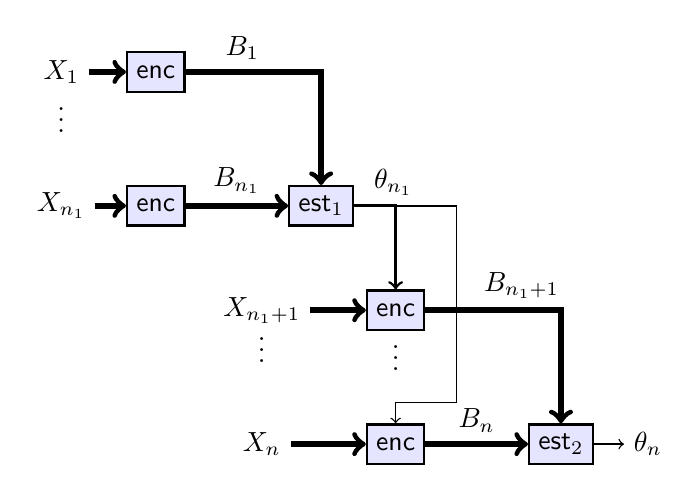
\begin{tikzpicture}[node distance=2cm,auto]
  \node at (0,0) (source) {$X_1$} ;
  \node[int1, right of = source, node distance = 1.2cm] (enc1) {$\enc$};  
\draw[->,line width = 2pt] (source) -- (enc1); 

% \node[below of = source, node distance = 1cm] (source2) {$X_2$};
%\node[int1, right of = source2, node distance = 1.2cm] (enc2) {Enc};  
%\draw[->,line width = 2pt] (source2) -- (enc2); 

\node[below of = source, node distance = 1.7cm] (source3) {$X_{n_1}$};
\node[int1, right of = source3, node distance = 1.2cm] (enc3) {$\enc$};  

\draw[->,line width = 2pt] (source3) -- (enc3); 

\node[below of = source, node distance = 0.5cm] {$\vdots$};

\node[int1, right of = enc3, node distance = 2.1cm ] (est) {$\est_1$};

\draw[->,line width = 2pt] (enc1) -| node[above, xshift = -1cm] (mes1) {$B_1$} (est);   

%\draw[->,line width = 2pt] (enc2) -| node[above, xshift = -1cm] (mes2) {$B_2$} (est);   

\draw[->,line width = 2pt] (enc3) -- node[above, xshift = 0cm]  {$B_{n_1}$} (est);   

\node[below right = 0.75 and 1.5 of source3] (sourceB) {$X_{n_1 +1}$} ;
\node[int1, right of = sourceB, node distance = 1.7cm] (enc1B) {$\enc$};  
\draw[->,line width = 2pt] (sourceB) -- (enc1B); 

\node[below of = sourceB, node distance = 1.7cm] (source3B) {$X_n$};
\node[int1, right of = source3B, node distance = 1.7cm] (enc3B) {$\enc$};  
\draw[->,line width = 2pt] (source3B) -- (enc3B); 
\node[below of = sourceB, node distance = 0.4cm] {$\vdots$};

\node[int1, right of = enc3B, node distance = 2.1cm ] (estB) {$\est_2$};

\draw[->,line width = 2pt] (enc1B) -| node[above, xshift = -0.5cm] {$B_{n_1+1}$} (estB);
\draw[->,line width = 2pt] (enc3B) -- node[above] {$B_n$} (estB);

\draw[->,line width = 1pt] (est.east) node[above, xshift  =0.5cm] {${\theta}_{n_1}$} -| (enc1B.north);

%\draw[->,line width = 1pt] (enc1B) -- (enc3B);

\draw[->,line width = 0.5pt] (est.east) -| +(1.3,-0.5) -- +(1.3,-2.5) -| (enc3B.north);

%\draw[->,line width = 1pt] (enc1B)  -- node[right] {${\theta}_{n_1}$} (enc3B);

\draw[->,line width = 0.5pt] (estB) -- +(0.8,0) node[right] {${\theta}_n$};
\node[below of = enc1B, node distance = 0.5cm] {$\vdots$};

\end{tikzpicture}
\end{center}
\caption{Distributed encoding with a single interaction: The estimation obtained from the first $n_1$ bits in a distributed manner is to obtain another $n-n_1$ bits in a distributed manner. 
\label{fig:one_round}
}
\end{figure}

\subsection{Maximal Efficiency using One Round of Threshold Adaptation}
In Section~\ref{sec:preliminary} we considered an estimator that is based on binary messages of the form 
\[
B_i = \mathbf 1_{X_i > \theta_0},\qquad i=1,\ldots,n,
\]
and deduced that it is asymptotically normal with variance $1/\eta(\theta-\theta_0)$.
%
We now show that a similar encoding leads to an asymptotically normal estimator attaining the lower variance bound $1/\eta(0)$, provided we allow to  update the threshold value $\theta_0$ based on previously observed bits at least once. 
%
In this procedure we separate the sample into two disjoint sets: $X_1,\ldots,X_{n_1}$ and $X_{n_1+1},\ldots,X_n$ for some $n_1 < n$.
We first use the estimator \eqref{eq:estimator_naive} to obtain an estimate ${\theta}_{n_1}$ based on $B_1,\ldots,B_{n_1}$, and then use ${\theta}_{n_1}$ as the new threshold value to obtain messages $B_{n_1+1}, \ldots, B_n$. Figure~\ref{fig:one_round} illustrates a diagram of this procedure. 
%
The specific encoding and estimation scheme, as well as its asymptotic performance, are given by the following theorem:
\begin{thm}
For $i=1,\ldots,n$ set
\[
B_i = \begin{cases}
 \mathbf 1_{X_i \geq \theta_0} & i = 1,\ldots,n_1, \\
 \mathbf 1_{X_i \geq {\theta}_{n_1} }& i={n_1+1,\ldots,n},
\end{cases}
\]
where $n = n_1+ n_2$ and 
\[
{\theta}_{n_1} \triangleq \theta_0 + F^{-1}\left(
\frac{1}{n_1} \sum_{i=1}^{n_1} B_i 
 \right).
\] 
Let 
\[
{\theta}_{n_2}  = {\theta}_{n_1} +  F^{-1} \left( \frac{1}{n_2} \sum_{i=n_1+1}^{n_2} B_i \right)
\]
and assume that $n_1(n) \rightarrow \infty$ and $n_1(n)/n \rightarrow 0$. Then:
\begin{align*}
 \sqrt{n} \left( {\theta}_{n_2} - \theta  \right) \overset{d}{\longrightarrow}  \Ncal\left( 0, 1/\eta(0) \right).
\end{align*}
\end{thm}
%
%
\begin{proof}
For $t\in \mathbb R$, set
\[
p_{n_2}(t) \triangleq \frac{1}{n_2} \sum_{i=n_1+1}^{n} \mathbf 1_{X_i \geq t}. 
\]
From the central limit theorem
\begin{align*}
& \sqrt{n} \left( p_{n_2}(t) - F( \theta - t) \right)  = \sqrt{\frac{n}{n_2}} \sqrt{n_2} \left(  p_{n_2}(t) - F(\theta - t) \right) \\
& \overset{d}{\rightarrow} \Ncal\left( 0, V(t) \right),
\end{align*}
where
\[
V(t) \triangleq F(\theta - t) F \left( t - \theta\right). 
\]
Applying the delta method to $p_{n_2}(t)$ with $g(x) = F^{-1}(x)$ implies
\begin{align*}
& \sqrt{n} \left( t + F^{-1}(\hat{p}_{n_2}(t)) - \theta \right) \\
&= \sqrt{n} \left( g(\hat{p}_{n_2}(t)) - g \left(F(\theta-t) \right)  \right) \\
& \overset{d}{\to} \Ncal\left(0, 
1/\eta(\theta-t) \right).
\end{align*}
%where this convergence is uniform in $t$ since all moments of $F^{-1}(\hat{p}_{n_2})$ exists. 
On the other hand, by the law of large numbers,
\[
p_{n_1} \triangleq \frac{1}{n_1} \sum_{i=1}^{n_1} B_i \overset{a.s.}{\rightarrow} F(\theta - \theta_0),
\]
so that ${\theta}_{n_1}$ converges almost surely to $\theta$ as $n$ goes to infinity and thus 
\[
\eta( {\theta}_{n_1}-\theta) \overset{a.s.}{\rightarrow} \eta(0). 
\]
Finally,
\begin{align*}
& \sqrt{n}\left({\theta}_{n_2} - \theta\right) \\
& = \sqrt{n} \left( {\theta}_{n_1} + F^{-1}(\hat{p}_{n_2}({\theta}_{n_1})) - \theta \right)  \\
& \overset{d}{\to} \Ncal\left( 0, 
1/\eta(0) \right) 
\end{align*}
by Slutsky's theorem.
\end{proof}
%

\begin{figure}
\begin{center}
\begin{tikzpicture}[scale = 0.6]
\begin{axis}[
width=10cm, height=6cm,
xmin = 0, xmax=800, 
restrict y to domain = 0:3,
ymin = 0,
ymax = 3.4,
samples=10, 
xlabel= $n$,
ylabel = {$n\mathbb E \left[\left(\theta - {\theta}_n \right)^2 \right]$},
%xtick={-3,-2,-1,0,1,2,3},
%xticklabels={-3,-2,-1,0,1,2,3},
ytick={0,1,1.57},
yticklabels={0,1,$\pi/2$},
line width=1.0pt,
mark size=1.5pt,
ymajorgrids,
xmajorgrids,
legend style= {at={(1,1)},anchor=north east,draw=black,fill=white,align=left}
]

\addplot[color = blue, solid, smooth] plot table [x = itr, y = SGD, col sep=comma] {./SimRes/sim_res_nMonte5000.csv};
\addlegendentry{asymptotically optimal};

%\addplot[color = red, solid, smooth] plot table [x = itr, y = Bayes, col sep=comma] {./SimRes/sim_res_nMonte5000.csv};\addlegendentry{one step optimal};

\addplot[color = red, solid, smooth] plot table [x = itr, y = split, col sep=comma] {./SimRes/sim_res_nMonte5000.csv};
\addlegendentry{single interaction};

\end{axis}
\end{tikzpicture}
%\begin{tikzpicture}
%\node at (0,0) {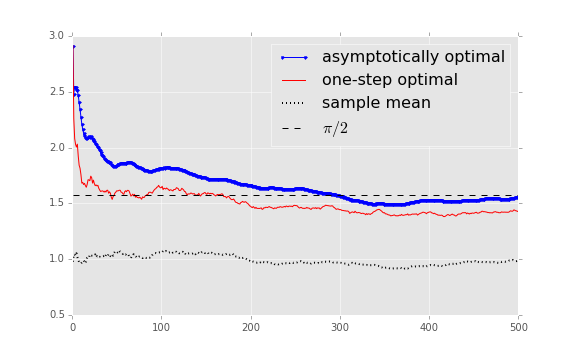
\includegraphics[scale=0.4]{one_bit_adpative}};
%\node[rotate = 90, scale = 0.7] at (-3.8,0) {$n \mathbb E \left({\theta}_n - \theta \right)^2$};
%\node[scale = 0.7] at (0,-2.4) {$n$};
%\end{tikzpicture}
\caption{Normalized empirical risk versus number of samples $n$ for $10,000$ Monte Carlo trials with $f(x)$ the standard normal density. In each trial, $\theta$ is chosen uniformly over the interval $(-1.64,1.64)$. The single interaction strategy uses $n_1 = \lfloor \sqrt{n} \rfloor$ samples for its first stage. 
\label{fig:adaptive_error}  }
\end{center}
\end{figure}

\section{Distributed Estimation \label{sec:distributed}}
In this section, we now consider the distributed encoding setting in Figure~\ref{fig:setup}-(iii) where  each one-bit message $B_i$ is only a function of its private sample $X_i$. In this case, the $i$th encoder is fully characterized its \emph{detection region}, defined as 
\[
A_i = \left\{ x \in \mathbb R \,:\, B_i(x) = 1 \right\}.
\]
Consequently, $B_i$ is of the form
\[
B_i = \begin{cases} 1 & X_i \in A_i, \\
-1 & X_i \notin A_i,
\end{cases} \quad i\in \mathbb N,
\]
where the detection region $A_i$ is a Borel set that is independent of $X_1,\ldots,X_n$.\par

As a first step, we provide conditions under which the messages $B_1,B_2,\ldots$ define a local asymptotic normal family. 

\begin{thm} \label{thm:LAN1}
For $n \in \mathbb N$ and $A_n \subset \mathbb R$,  define
\begin{equation}
\label{eq:precision_general}
L_n(A_1,\ldots,A_n;\theta) \triangleq \frac{1}{n} \sum_{i=1}^n \frac{ \left(\frac{d}{d \theta} \Prob(X_i \in A_i) \right)^2 }{ \Prob(X_i \in A_i)\left(1- \Prob(X_i \in A_i) \right) }. 
\end{equation}
Consider the following conditions:
\begin{itemize}
\item [(i)\,\,] The pdf $f(x)$ of $X_n-\theta$ is a log-concave, differentiable and symmetric density function such that $\eta(x)$ is unimodal.
\item[(ii)\,] $A_n$ is a finite union of disjoint intervals.
\item[(iii)] The limit 
\begin{equation}
\label{eq:LAN_lim}
\kappa(\theta) \triangleq \lim_{n\to \infty} L_n(A_1,\ldots,A_n; \theta)
\end{equation}
exists. 
\end{itemize}
For $i=1,\ldots,n$ set
\[
B_n = \begin{cases} 1 & X_n \in A_n, \\
-1 & X_n \notin A_n. 
\end{cases} 
\]
For any $\theta$, $f(x)$ and a sequence of sets $A_1,A_2,\ldots$ such that (i)-(iii) hold, and any $h\in \mathbb R$, we have
\begin{align*}
& \log  \frac{ \mathbb P_{\theta+h/\sqrt{n}} (B_1,\ldots,B_n) }{
\mathbb P_{\theta} (B_1,\ldots,B_n)} \\
& \overset{d}{\longrightarrow} \Ncal\left(-\frac{1}{2} h^2 \kappa(\theta), h^2 \kappa(\theta) \right).
\end{align*} 
\end{thm}

\begin{proof}
See Appendix~\ref{proof:thm:LAN1}. 
\end{proof}

Theorem~\ref{thm:LAN1} provides conditions under which $B_1,\ldots,B_n$ defines a LAN family with a precision parameter given by the limit in \eqref{eq:LAN_lim}. 
%
Among these conditions, (iii) is arguably the strongest and hardest to verify. As we show in Section~\ref{subsec:threshold} below, this condition is satisfied, for example, when $A_1, \ldots,A_n$ are half lines whose starting points are drawn independently from some probability measure on $\mathbb R$. Similar ideas imply that condition (iii) holds whenever we choose the intervals consisting each $A_i$ according to some pre-specified distribution. \par
%
An important conclusion of  Theorem~\ref{thm:LAN1} follows from the local asymptotic minimax property of estimators in LAN models \cite{van2000asymptotic}):
\begin{cor} \label{cor:LA_minimax}
Let ${\theta}_n$ be an estimator of $\theta \in \Theta$ from $B_1,\ldots,B_n$ with detection regions $A_1,\ldots,A_n$ such that conditions (i)-(iii) of Theorem~\ref{thm:LAN1} hold. Then for any symmetric and quasi-convex function $L$, 
\begin{align*}
& \liminf_{c \to \infty} \liminf_{n \to \infty} \sup_{\tau\,:\,|\theta-\tau| \leq \frac{c}{\sqrt{n} }}  \mathbb E \left[ L\left( \sqrt{n}({\theta}_{n} - \tau) \right) \right]
\\
& \qquad \qquad \qquad \qquad \geq \mathbb E \left[ L (Z/\sqrt{\kappa(\theta)}) \right],
\end{align*}
where $Z \sim \Ncal(0,1)$. In particular, for $L(x) = x^2$,
\begin{align*}
\liminf_{c \to \infty} \liminf_{n \to \infty} \sup_{\tau\,:\,|\theta-\tau| \leq \frac{c}{\sqrt{n} }}  n \mathbb E  \left( {\theta}_{n} - \tau \right)^2 \geq 1/\kappa(\theta).
\end{align*}
\end{cor}
%
Corollary~\ref{cor:LA_minimax} says that when the messages define a LAN model, no estimator can attain MSE smaller than $1/\kappa(\theta)n + O(1/n)$ where $\kappa(\theta)$ is the precision parameter of the model at $\theta$. This fact poses the upper bound of $\kappa(\theta)\sigma^2$ for the ARE of estimators in such models. \par

Next, we show that under LAN no estimator can attain the optimal ARE of $\eta(0)\sigma^2$ uniformly for all $\theta \in \Theta$.

\subsection{Non-existence of a Uniformly Optimal Strategy}
We now show that under LAN models, the optimal minimal risk $1/\eta(0)$ can only be attained at a finite number of points within $\Theta$. This fact implies in particular that, unlike in the adaptive setting, no distributed estimation scheme has ARE of $\eta(0)\sigma^2$ for all $\theta \in \Theta$. 

\begin{thm} \label{thm:non_existence}
Under conditions (i)-(iii) in Theorem~\ref{thm:LAN1}, assume that each $A_i$ is a union of at most $K$ intervals. The number of points $\theta \in \Theta$ satisfying $\kappa(\theta) = \eta(0)$ is at most $2K$. 
\end{thm}

\begin{proof}
See Appendix~\ref{proof:thm:non_existence}.
\end{proof}

We next consider the case where each detection region is a half-open interval, i.e., the $i$th message is obtained by comparing $X_i$ against a single threshold. As we explain next, the existence of a density for the sequence of thresholds is enough to establish local asymptotic normality and leads to a closed form expression for the precision parameter and the ARE.  

%In the adaptive setting, it follows from Theorem~\ref{thm:sgd} that messages of this kind with appropriately chosen thresholds lead to an estimator with the optimal ARE of $\eta(0)sigma^2$. However, Theorem~\ref{thm:non_existence} implies that such ARE can only be attained for a negligible subset of the parameter space. As we shall see next, messages obtained via a comparison against a sequence of thresholds cannot attain the optimal efficiency one more than a single point of $\Theta$. 

\subsection{Threshold Detection \label{subsec:threshold}}
Assume now that each $B_i$ is of the form
\begin{equation}
\label{eq:threshold_message}
B_i = \sgn(t_i - X_i) = \begin{cases} 1 & X_i< t_i, \\
-1 & X_i > t_i,
\end{cases}  
\end{equation}
where $t_i\in\mathbb R$ is the \emph{threshold} of the $i$th encoder. In other words, the detection region of $B_i$ is $A_i = (t_i,\infty)$ and $\mathbb P(X_i \in A_i) = F \left( B_i(t_i-\theta) \right)$. It follows that
\begin{equation}
L_n(A_1,\ldots,A_n;\theta) = \frac{1}{n} \sum_{i=1}^n \frac{ \left(f(t_i-\theta) \right)^2 }{F\left(t_i-\theta \right) F\left(\theta - t_i \right) }  = \frac{1}{n} \sum_{i=1}^n \eta(t_i - \theta).
\label{eq:Ln_threshold}
\end{equation}
A natural condition for the existence of the limit \eqref{eq:Ln_threshold} as $n\to \infty$ is that the empirical distribution of the threshold values converges to a probability measure. Specifically, for an interval $I \subset \mathbb R$ define
\[
\lambda_n(I) = \frac{ \card \left( I \cap \{t_1,t_2,\ldots \} \right)}{n}. 
\]
Theorem~\ref{thm:LAN1} implies:
\begin{cor} \label{cor:LAN_thresh}
Let $\{t_n\}_{n=1}^\infty$ be a sequence of threshold values such that $\lambda_n$ converges (weakly) to a probability measure $\lambda(dt)$ on $\mathbb R$. Then $\left\{ B_i = \sgn(X_i - t_i) \right\}_{i=1}^n$ is a LAN family with precision parameter
\[
\kappa(\theta) = \int_{\mathbb R} \eta(t-\theta) \lambda(dt). 
\]
\end{cor}
The condition that $\lambda_n$ converges to a probability measure is satisfies, for example, whenever the $t_1,\ldots,t_n$s are drawn independently from a probability distribution $\lambda(dt)$ on $\mathbb R$. \par
Due to local asymptotic normality of $\{B_n\}_{n=1}^\infty$, the maximum likelihood estimator (ML) of $\theta$ from $B_1,\ldots,B_n$, denoted here by 
${\theta}^{ML}_n$, is local asymptotic minimax in the sense that 
\[
\sqrt{n} \left( {\theta}^{ML}_n - \theta \right) \overset{d}{\longrightarrow} \mathcal{N} \left(0, 1/\kappa(\theta) \right). 
\]
It follows that when the density of the threshold values converges to a probability measure, the ARE of the ML estimator is $\kappa(\theta)\sigma^2$, and this ARE is maximal with respect to all local alternative estimators for $\theta$. We note that ${\theta}^{ML}_n$ is given by the root of 
\begin{equation}
\label{eq:ML}
\sum_{i=1}^n B_i \frac{f \left( t_i-\theta\right) }{F \left(B_i  (t_i-\theta)\right) },  
\end{equation}
which is the derivative of the log-likelihood function. This root is unique since the log-likelihood function is concave. Furthermore, for any $n \in \mathbb R$, we have that ${\theta}^{ML}_n  \in [t_{(1)}, t_{(n)}]$ where $t_{(i)}$ denotes the $i$th element of $\{t_1,t_2\ldots\}$. Therefore, if $\{t_1,t_2\ldots\}$ is bounded (for example $\{t_1,t_2\ldots\} \subset \Theta$), then 
\[
\lim_{n\to \infty} n \ex{\left({\theta}^{ML}_n - \theta \right)^2}  = 1/\kappa(\theta), 
\] 
so that the ML estimator attains the local asymptotic MSE of Corollary~\ref{cor:LA_minimax}. \par
%
Since $\eta(x)$ attains its maximum at the origin, we conclude that
\[
\kappa(\theta) \leq \sup_{t\in \mathbb R} \eta \left( t-\theta\right) = \eta(0).
\]
This upper bound on $\kappa(\theta)$ implies that the ARE of any distributed estimator based on a sequence of threshold detectors does not exceed $\eta(0)\sigma^2$, a fact that agrees with the lower bound under adaptive estimation derived in Theorem~\ref{thm:adpative_lower_bound}. 
%
This upper bound on $\kappa(\theta)$ is attained only when $\lambda$ is the mass distribution at $\theta$. Since $\theta$ is apriori unknown, we conclude that estimation in the distributed setting using threshold detection is strictly sub-optimal compared to the adaptive setting. In other words, the ability to choose the threshold values in an adaptive manner based on previous messages strictly improves relative efficiency compared to a non-adaptive threshold selection.  \par

%We conclude that when the density of the threshold values converges to a probability measure, the ARE of the ML is $\kappa(\theta)$, and this ARE is maximal with respect to all local alternative estimators for $\theta$. 

%
We conclude this section by considering the density of the threshold values that maximizes the ARE $\kappa(\theta)$ under the worst choice of $\theta \in \Theta$.

\subsection{Minimax Threshold Density}
The distribution $\lambda(dt)$ that maximizes $\kappa(\theta)$, and thus minimizes $1/\kappa(\theta)$, over the worst choice of $\theta$ in $\Theta = [-T,T]$ is given as the solution to the following optimization problem:
\begin{align}
\label{eq:var_cvx_minimax}
\begin{split}
\mathrm{maximize} \quad &  \inf_{\theta \in [-T,T]} \int \eta(t-\theta) \lambda(dt)
\\ 
\mathrm{subject~to} 
\quad & \lambda(dt)\geq 0,\quad \int \lambda(dt) \leq 1. 
\end{split}
\end{align}
The objective function in \eqref{eq:var_cvx_minimax} is concave in $\lambda(dt)$ and hence this problem can be solved using a convex program. We denote by $\kappa^\star(T)$ the maximal value of \eqref{eq:var_cvx_minimax} and by $\lambda^\star(dt)$ the density that achieves this maximum.  
%
%By discretizing the interval $[-b,b]$ using $N_\theta$ values $\theta_1,\ldots,\theta_{N_\theta}$ and the real line using $N_\lambda$ values $\lambda_1,\ldots,\lambda_{N_\lambda}$, the discrete version of \eqref{eq:var_cvx_minimax} is the following linear program (LP) in the variables $K \in \mathbb R$ and $\lambda \in \mathbb R^{N_\lambda}$:
%\begin{align}
%\label{eq:cvx_minimax}
%\begin{split}
%\mathrm{maximize} \quad &  K \\ 
%\mathrm{subject~to} 
%\quad &  K \leq \mathbf H\lambda \\
%& \lambda \geq 0,\quad   \mathbf 1^T\lambda  \leq 1,
%\end{split}
%\end{align}
%where $\mathbf H_{i,j} = \eta(t_i - \theta_j)$, $i=1,\ldots,N_\lambda$, $j = 1,\ldots,N_\theta$. 
%\begin{rem}
%The number of variables in \eqref{eq:cvx_minimax} is $N_\lambda+1$ and number of constraints is $1 + N_\lambda + N_\theta$. Since an LP has an optimal solution at which the number of constraints for which equality holds is no smaller than the number of variables \cite{papadimitriou1998combinatorial}, there exists an optimal $\lambda$ with support over no more than $N_{\theta}$ points. Therefore, in approximating the solution of \eqref{eq:var_cvx_minimax} using 
%\eqref{eq:cvx_minimax}, it is enough to take $N_\lambda = N_\theta$.
%\end{rem} 

Figure~\ref{fig:minimax_support} illustrates an approximating to $\lambda^\star(dt)$ obtained by solving a discretized version of \eqref{eq:var_cvx_minimax} for the case when $f(x)$ is the normal density with variance $\sigma^2$. The minimal asymptotic risk $\kappa^\star(\theta)$ obtained this way is illustrated in Fig.~\ref{fig:minimax_ARE} as a function of the support size $T$. Also illustrated in these Figures is $\kappa_{\unif}$ which is the precision parameter corresponding to threshold values uniformly distribution over $\Theta = [-T,T]$, namely
\begin{align}
& \kappa_{\unif} \triangleq \min_{\theta \in [-T,T]} \frac{1}{2T}\int_{-T}^T \eta\left(t-\theta\right) dt \nonumber
 \\
& = 
\frac{1}{2T}\int_{-T}^{T} \eta\left(t\pm T\right) dt
= \frac{1}{2T}\int_{0}^{2T} \eta(t) dt  \label{eq:uniform_risk}. 
\end{align}
From Corollary~\ref{cor:LAN_thresh}, we conclude that the ARE under a uniform distribution is $\kappa_\unif \sigma^2$. \par

\begin{figure}
\begin{center}
\begin{tikzpicture}[scale = 0.55]
\begin{axis}[
width=8cm, height=6cm,
xmin = -0.5, xmax=0.5, 
restrict y to domain = 0:100,
ymin = 0,
ymax = 1,
samples=10, 
xlabel= {$dt$},
xtick={-0.5,0,0.5},
xticklabels={-$T$, 0, $T$},
title = {$\sigma/T = 1/2$},
ytick={0,0.1,1},
%ylabel = {$\lambda(dt)$},
yticklabels={0,0.1,1},
line width=1.0pt,
mark size=1.5pt,
ymajorgrids,
xmajorgrids,
legend style= {at={(1,1)},anchor=north east,draw=black,fill=white,align=left}
]
\addplot[color = blue, smooth, mark = o ] plot table [col sep=comma] {./Figs/minmax_lmd_b0.5_sig0.5.csv};

\addplot[color = black!30!green, smooth, dashed] plot table [x = x, y  = z,col sep=comma] {./Figs/minimax_th_b0.5_sig0.5.csv};

\addplot[color = red, smooth] plot table [x = x, y  = y,col sep=comma] {./Figs/minimax_th_b0.5_sig0.5.csv};

\end{axis}
\end{tikzpicture}
%
\begin{tikzpicture}[scale = 0.55]
\begin{axis}[
width=8cm, height=6cm,
xmin = -0.5, xmax=0.5, 
restrict y to domain = 0:100,
ymin = 0,
ymax = 0.6,
samples=10, 
xlabel= {$dt$},
title = {$\sigma/T = 1/5$},
xtick={-0.5,0,0.5},
xticklabels={-$T$, 0, $T$},
ytick={0,0.5},
ylabel = {$\lambda(dt)$},
yticklabels={0,0.5},
line width=1.0pt,
mark size=1.5pt,
ymajorgrids,
xmajorgrids,
legend style= {at={(1,1)},anchor=north east,draw=black,fill=white,align=left}
]
\addplot[color = blue, smooth, mark = o ] plot table [col sep=comma] {./Figs/minmax_lmd_b0.5_sig0.2.csv};

\addplot[color = black!30!green, smooth, dashed] plot table [x = x, y  = z,col sep=comma] {./Figs/minimax_th_b0.5_sig0.2.csv};

\addplot[color = red, smooth] plot table [x = x, y  = y,col sep=comma] {./Figs/minimax_th_b0.5_sig0.2.csv};

\end{axis}
\end{tikzpicture}
%
\begin{tikzpicture}[scale = 0.55]
\begin{axis}[
width=8cm, height=6cm,
xmin = -0.5, xmax=0.5, 
restrict y to domain = 0:100,
ymin = 0,
ymax = 0.3,
samples=10, 
xlabel= {$dt$},
xtick={-0.5,0,0.5},
title = {$\sigma / T = 1/10$},
xticklabels={-$T$, 0, $T$},
ytick={0,0.2},
%ylabel = {$\lambda(dt)$},
yticklabels={0,0.2},
line width=1.0pt,
mark size=1.5pt,
ymajorgrids,
xmajorgrids,
legend style= {at={(1,1)},anchor=north east,draw=black,fill=white,align=left}
]
\addplot[color = blue, smooth, mark = o ] plot table [col sep=comma] {./Figs/minmax_lmd_b0.5_sig0.1.csv};

\addplot[color = black!30!green, smooth, dashed] plot table [x = x, y  = z,col sep=comma] {./Figs/minimax_th_b0.5_sig0.1.csv};

\addplot[color = red, smooth] plot table [x = x, y  = y,col sep=comma] {./Figs/minimax_th_b0.5_sig0.1.csv};

\end{axis}
\end{tikzpicture}
%
\begin{tikzpicture}[scale = 0.55]
\begin{axis}[
width=8cm, height=6cm,
xmin = -0.5, xmax=0.5, 
restrict y to domain = 0:100,
ymin = 0,
ymax = 0.15,
samples=10, 
xlabel= {$dt$},
title = {$\sigma / T = 1/20$},
xtick={-0.5,0,0.5},
xticklabels={-$T$, 0, $T$},
ytick={0,0.1},
ylabel = {$\lambda(dt)$},
yticklabels={0,0.1},
line width=1.0pt,
mark size=1.5pt,
ymajorgrids,
xmajorgrids,
legend style= {at={(1,1)},anchor=north east,draw=black,fill=white,align=left}
]
\addplot[color = blue, smooth, mark = o ] plot table [x = x, y  = y,col sep=comma] {./Figs/minmax_lmd_b0.5_sig0.05.csv};

\addplot[color = black!30!green, smooth, dashed] plot table [x = x, y  = z,col sep=comma] {./Figs/minimax_th_b0.5_sig0.05.csv};

\addplot[color = red, smooth] plot table [x = x, y  = y,col sep=comma] {./Figs/minimax_th_b0.5_sig0.05.csv};


%\addlegendentry{$\frac{\sigma^2}{\sigma_\theta^2} = 1$};
\end{axis}
\end{tikzpicture}

\caption{\label{fig:minimax_support}
Optimal threshold density $\lambda^\star(dt)$ (blue) that maximizes the ARE for $f(x) = \Ncal(\theta,\sigma^2)$ and $\theta \in \Theta = [-T,T]$.
%
The continuous curve (red) represents the reciprocal of the asymptotic risk for at a fixed $\theta \in \Theta$ under the optimal density, so the minimax risk is the inverse of its minimal value. The dashed curve (green) is the reciprocal of the asymptotic risk for a fixed $\theta$ under a uniform distribution of threshold values over $\Theta$, hence its minimal value is the inverse of \eqref{eq:uniform_risk}. }
\end{center}
\end{figure}


\begin{figure}
\begin{center}
\begin{tikzpicture}[scale = 1]
\begin{axis}[
width=8cm, height=6cm,
xmax=2.5, 
xmode = log,
restrict y to domain = 0:100,
ymin = 0,
ymax = 1,
samples=1, 
xlabel= {$\sigma/T$},
%xtick={-0.5,0,0.5},
%xticklabels={-$$, 0, $b$},
ytick={0,0.637,1},
yticklabels={0,$2/\pi$,1},
ylabel = {$\ARE$},
line width=1.0pt,
mark size=1.5pt,
ymajorgrids,
xmajorgrids,
legend style= {at={(1,1)},anchor=north east,draw=black,fill=white,align=left}
]
\addplot[color = red, smooth, line width = 1pt] plot table [x = x, y = y, col sep=comma] {./Figs/minmax_ARE_b0.5.csv};
\addlegendentry{optimal threshold density};

\addplot[color = black!35!green, smooth, dashed, line width = 1pt] plot table [x = x, y = z, col sep=comma] {./Figs/minmax_ARE_b0.5.csv};
\addlegendentry{uniform threshold desnity};
\end{axis}
\end{tikzpicture}
\caption{\label{fig:minimax_ARE} Minimax ARE versus $\sigma/T$ for $f(x) = \Ncal(\theta,\sigma^2)$  and $\theta \in \Theta = [-T,T]$. The dashed curve (green) is the ARE under a uniform threshold density over $\Theta$ given by $K_{\unif}\sigma^2$, where $\kappa_{\unif}$ is given by \eqref{eq:uniform_risk}. }.
\end{center}
\end{figure}


%We have seen that using threshold detection, an ARE $\eta(0)\sigma^2$ can only be attained at a single point in $\Theta$. Next, we prove that with any set of messages obtained via a distributed strategy, there exists at least one $\theta \in \Theta$ such that the estimator of $\theta$ has ARE strictly smaller than $\eta(0)\sigma^2$. 

\begin{figure}
\begin{center}
\begin{tikzpicture}[scale = 0.55]
\begin{axis}[
width=8cm, height=6cm,
xmin = -0.5, xmax=0.5, 
restrict y to domain = 0:100,
ymin = 0,
ymax = 1,
samples=10, 
xlabel= {$dt$},
xtick={-0.5,0,0.5},
xticklabels={-$b$, 0, $b$},
title = {$\sigma/\sigma_{\theta} = 1$},
ytick={0,1},
%ylabel = {$\lambda(dt)$},
yticklabels={0,1},
line width=1.0pt,
mark size=1.5pt,
ymajorgrids,
xmajorgrids,
legend style= {at={(1,1)},anchor=north east,draw=black,fill=white,align=left}
]
\addplot[color = blue, smooth, mark = o ] plot table [col sep=comma] {./Figs/unif_Bayes_lmd_b0.5_sig1.csv};
%\addlegendentry{$\frac{\sigma^2}{\sigma_\theta^2} = 1$};
\end{axis}
\end{tikzpicture}
%
\begin{tikzpicture}[scale = 0.55]
\begin{axis}[
width=8cm, height=6cm,
xmin = -0.5, xmax=0.5, 
restrict y to domain = 0:100,
ymin = 0,
ymax = 1,
samples=10, 
xlabel= {$dt$},
title = {$\sigma/\sigma_{\theta} = 2$},
xtick={-0.5,0,0.5},
xticklabels={-$b$, 0, $b$},
ytick={0,1},
ylabel = {$\lambda(dt)$},
yticklabels={0,1},
line width=1.0pt,
mark size=1.5pt,
ymajorgrids,
xmajorgrids,
legend style= {at={(1,1)},anchor=north east,draw=black,fill=white,align=left}
]
\addplot[color = blue, smooth, mark = o ] plot table [col sep=comma] {./Figs/unif_Bayes_lmd_b0.5_sig2.csv};
%\addlegendentry{$\frac{\sigma^2}{\sigma_\theta^2} = 1$};
\end{axis}
\end{tikzpicture}
%
\begin{tikzpicture}[scale = 0.55]
\begin{axis}[
width=8cm, height=6cm,
xmin = -0.5, xmax=0.5, 
restrict y to domain = 0:100,
ymin = 0,
ymax = 1,
samples=10, 
xlabel= {$dt$},
xtick={-0.5,0,0.5},
title = {$\sigma/\sigma_{\theta} = 3$},
xticklabels={-$b$, 0, $b$},
ytick={0,1},
%ylabel = {$\lambda(dt)$},
yticklabels={0,1},
line width=1.0pt,
mark size=1.5pt,
ymajorgrids,
xmajorgrids,
legend style= {at={(1,1)},anchor=north east,draw=black,fill=white,align=left}
]
\addplot[color = blue, smooth, mark = o ] plot table [col sep=comma] {./Figs/unif_Bayes_lmd_b0.5_sig3.csv};
%\addlegendentry{$\frac{\sigma^2}{\sigma_\theta^2} = 1$};
\end{axis}
\end{tikzpicture}
%
\begin{tikzpicture}[scale = 0.55]
\begin{axis}[
width=8cm, height=6cm,
xmin = -0.5, xmax=0.5, 
restrict y to domain = 0:100,
ymin = 0,
ymax = 1,
samples=10, 
xlabel= {$dt$},
title = {$\sigma/\sigma_{\theta} = 4$},
xtick={-0.5,0,0.5},
xticklabels={-$b$, 0, $b$},
ytick={0,1},
ylabel = {$\lambda(dt)$},
yticklabels={0,1},
line width=1.0pt,
mark size=1.5pt,
ymajorgrids,
xmajorgrids,
legend style= {at={(1,1)},anchor=north east,draw=black,fill=white,align=left}
]
\addplot[color = blue, smooth, mark = o ] plot table [col sep=comma] {./Figs/unif_Bayes_lmd_b0.5_sig4.csv};
%\addlegendentry{$\frac{\sigma^2}{\sigma_\theta^2} = 1$};
\end{axis}
\end{tikzpicture}

\caption{\label{fig:opt_density}
Optimal threshold density $\lambda^\star(dt)$ that minimizes the asymptotic Bayes risk \eqref{eq:cvx_average} for a uniform prior with $\sigma/\sigma_\theta=1,2,3,4$, where $\sigma_\theta^2=b^2/3$ is the variance of the prior. 
}
\end{center}
\end{figure}

 We consider now the problem of minimizing the asymptotic Bayes risk $
R_{\pi,\lambda} \triangleq \mathbb E  K^{-1}(\theta)$ over all probability measures $\lambda(dt)$ with support in $\mathbb R$. This optimization problem can be written as follows:
\begin{align}
\label{eq:cvx_average}
\begin{split}
\mathrm{minimize} \quad & R_{\pi,\lambda} =  \int \frac{\pi(d\theta)}{ \int \eta \left( t-\theta\right) \lambda(dt)}. \\ 
\mathrm{subject~to} \quad & \lambda(dt)\geq 0,\quad \int \lambda(dt) =1. 
\end{split}
\end{align}
We denote by $R^\star_{\pi}$ the minimal value of the objective function in \eqref{eq:cvx_average}. Since the function $x \rightarrow 1/x$ is convex for positive values, \eqref{eq:cvx_average} defines a convex optimization problem in $\lambda$ whose solution depends on the prior $\pi$. The solution to this problem is approximated by considering $\lambda$ and $\pi$ over a discrete set. On Figure~\ref{fig:opt_density} we illustrate the solution to \eqref{eq:cvx_average} for the case of where $f(x)$ is the normal distributon ($P_X = \Ncal(\theta, \sigma^2)$) and the prior on $\theta$ is uniform over $\Theta = [-b,b]$. Figure~\ref{fig:dist_bound_uniform} illustrates the corresponding Bayes risk. 
\par
\begin{figure}
\begin{center}

\begin{tikzpicture}[scale = 1]
\begin{axis}[
width=8cm, height=6cm,
xmin = 0, xmax=2, 
restrict y to domain = 0:100,
ymin = 0,
ymax = 10,
samples=1, 
xlabel= {$\sigma/\sigma_\theta$},
%xtick={-0.5,0,0.5},
%xticklabels={-$$, 0, $b$},
ytick={0,1.5708,5},
yticklabels={0,$\pi/2$,5},
ylabel = {$R_{\pi}^\star/\sigma^2$},
line width=1.0pt,
mark size=1.5pt,
ymajorgrids,
xmajorgrids,
legend style= {at={(1,1)},anchor=north east,draw=black,fill=white,align=left}
]
\addplot[color = red, smooth] plot table [x = x, y = Runif, col sep=comma] {./Figs/unif_Bayes_Risk.csv};
%\addlegendentry{$\frac{\sigma^2}{\sigma_\theta^2} = 1$};
\addplot[color = red, smooth, dashed, line width = 0.5pt] plot table [x = x, y = Rbound, col sep=comma] {./Figs/unif_Bayes_Risk.csv};
\addplot[color = black, dashed] {3.14159 / 2};
\end{axis}
\end{tikzpicture}
\caption{Asymptotic Bayes risk $R_{\pi}^\star$ in estimating the mean of a normal distribution ($P_X = \Ncal(\theta, \sigma^2)$ under an optimal threshold distribution $\lambda^\star$, when the prior $\pi$ is the uniform distribution over $\Theta = [-0.5,0.5]$. 
%
%versus $\sigma/\sigma_\theta = 2\sqrt{3}\sigma$.
The distribution $\lambda^\star$ is the minimizer of \eqref{eq:cvx_average}. It is illustrated for various cases in Fig.~\ref{fig:opt_density}. The dashed curve represents the upper bound \eqref{eq:upper_bound}. 
\label{fig:dist_bound_uniform}  }
\end{center}
\end{figure}

As can be seen in Fig.~\ref{fig:opt_density} for the case $P_X = \Ncal(\theta ,\sigma^2)$ and a uniform $\pi$, when the radius of $\Theta$ is small compared to $\sigma$, the optimal distribution $\lambda^\star$ is a mass distribution. In this case, the ML estimator reduces to the estimator ${\theta}_n$ of \eqref{eq:estimator_naive}. As the following proposition shows, the Bayes risk for this choice of $\lambda$ is maximal, and thus provides an upper bound on the Bayes risk under any $\lambda$. 
 \eqref{eq:cvx_average}. 
\begin{prop}\label{prop:upper_bound}
For any prior $\pi(d\theta)$ and $\theta_0$ in the support of $\eta(x)$ we have
\begin{equation} 
\label{eq:upper_bound}
R_\pi^\star  \leq 
 \int \frac{\pi(d\theta)}{\eta \left( \theta_0 - \theta \right)},
\end{equation}
Furthermore, assuming that $\theta_0 = \mathbb E \theta$ and that $\pi$ has a finite third moment $\sigma_\theta^3$, we have: 
\begin{equation}
\label{eq:bound_Taylor}
R^\star_\pi \leq \frac{1}{4 f^2(0)} + \left(\frac{1}{4 f^2(0)} \frac{-f''(0)}{f(0)} -1 \right) \sigma_\theta^2 + O(\sigma_\theta^3).
\end{equation}
\end{prop}
\begin{proof}
The function $x \rightarrow 1/x$ is convex for positive values, hence Jensen's inequality implies
\[
\left( \int \eta \left( t-\theta\right) \lambda(dt) \right)^{-1}  \leq \int  \frac{ \lambda(dt)}{ \eta \left( t-\theta\right)  }. 
\]
Therefore, the expected value of $\kappa^{-1}(\theta)$ satisfies
\begin{align}
\ex{  \frac{1}{\kappa(\theta)}}  \leq \int \int \frac{\pi(d\theta) \lambda(dt) }{\eta \left( t - \theta \right)}. \label{eq:upper_bound_proof}
\end{align}
The bound \eqref{eq:upper_bound} is obtained by taking $\lambda$ to be a mass distribution at any $\theta_0$ in the support of $\eta(x)$. Finally, \eqref{eq:bound_Taylor} is obtained by expanding $1/\eta(x)$ to a third order Taylor series around zero
%\[
%1/\eta(x) = \frac{1}{4f^2(0)}  + \left(\frac{1}{4 f^2(0)} \frac{-f''(0)}{f(0)} -1 \right)  x^2 + O(x^3),
%\]
and taking its expectation with respect to $\pi$ at $x=\theta_0-\theta$. 
\end{proof}
We note that the function $1/\eta(x)$ is quasi-convex and symmetric around zero, so the choice $\theta_0 = \ex{ \theta}$ minimizes the RHS of \eqref{eq:upper_bound} among all $\theta_0$ in the support of $\eta(x)$.\par
The bound \eqref{eq:upper_bound} is not trivial as long as the integral in the RHS of \eqref{eq:upper_bound} is finite, i.e., whenever the tail of $\pi(\theta)$ vanishes fast enough compared to $\eta(x)$. The expansion \eqref{eq:bound_Taylor} implies that this bound becomes tight whenever the support of the optimal distribution is a mass distribution at $\mathbb E \theta$, in which case the expected value of $\kappa^{-1}(\theta)$ approaches $1/\eta(0) = 1/4f^2(0)$. 

\begin{example} \label{ex:bound}
In the normal case $P_X = \Ncal(\theta, \sigma^2)$, the bound in \eqref{eq:bound_Taylor} implies 
\[
\frac{R^\star_\pi}{\sigma^2}  \leq \frac{\pi}{2} + \left( \frac{\pi}{2} -1 \right) \left( \frac{ \sigma_\theta}{\sigma} \right)^2 + O \left(  \frac{\sigma_\theta} { \sigma} \right)^3. 
\]
It follows that the ARE approaches its maximal value of $2/\pi$ whenever $\sigma_\theta/\sigma$ is small. The exact value of \eqref{eq:upper_bound} in this case, as well as the Bayes ARE with the optimal threshold density $\lambda^\star$ for a uniform $\pi$, are illustrated in Fig.~\ref{fig:dist_bound_uniform}. 
%i.e., each encoder simply reports "$1$" or "$-1$" whenever $X_i$ is larger or smaller than $\theta_0$, respectively. Intuitively, an accurate estimation of $\theta$ in this case is possible only if a sufficient mix of ''$1$''s and ''$-1$''s is obtained from the sample. When $\sigma_\theta^2$ is high compared to $\simga^2$, one of the events $"1"$ or "$-1"$ becomes too rare to
\end{example}

\section{Conclusions \label{sec:conclusions}}
We considered the MSE risk in estimating the mean of a symmetric and log-concave distribution from a sequence of bits, where each bit is obtained by encoding a single sample from this distribution. 
%
In an adaptive encoding setting, we showed that no estimator can attain asymptotic relative efficiency (ARE) larger than that of the median of the samples. We also showed that this bound is tight by presenting two adaptive encoding and estimation procedures that are as efficient as the median. 
%We also characterized the one-step optimal scheme in this adaptive setting, i.e., the scheme that minimizes the risk given any set of previously obtained bits.
\par
In the distributed setting we provided conditions for local asymptotic normality of the encoded samples, which implies asymptotic minimax bound on both the risk and ARE. 
%
We conclude that under such conditions, the optimal estimation performance derived for the adaptive case can only be attained over a finite number of points, i.e., no scheme is uniformly optimal in the distributed setting. 
%
We further considered the special case of messages obtained by comparing against a prescribed sequence of thresholds. We characterized the performance of the optimal estimator from such messages using the density of these thresholds, and consider the threshold density that minimizes the minimax risk. 


%\section*{ACKNOWLEDGMENT}
%This research is supported in parts by...
%Tsachy Weissman, Stefano Rini, Robert Gray.


\onecolumn 

\appendix

\section{}

\subsection{Proof of Proposition~\ref{prop:ceo_lower_bound}
\label{app:proof:prop_ceo_lower_bound}}

First, we note that when $f(x) = \Ncal(0,\sigma^2)$ and $\pi(\theta) = \Ncal(0,\sigma_\theta^2)$, our distributed setting reduces to the Gaussian CEO problem with $R_1=\ldots = R_n =1$ and $k=1$. Therefore, any MSE attained in our distributed setting is also attained by the CEO and thus the optimal CEO strategy (with arbitrary $k$) provides a lower bound to the MSE in our setting. \\

Consider the minimal MSE $D^\star$ in the Gaussian CEO setting with $L$ observers and under a total sum-rate $R_\Sigma = R_1 + \ldots +R_L$
from \cite[Eq. 10]{chen2004upper}:
\begin{equation} \label{eq:ceo_optimal_sumrate}
R_{\Sigma} = \frac{1}{2} \log^+ \left[ \frac{\sigma_\theta^2}{D^\star} \left( \frac{D^\star L}{ D^\star L - \sigma^2 + D^\star \sigma^2 / \sigma_\theta^2 }\right)^L  \right].
\end{equation}
For the special case of $R_\Sigma = n$ and $L=n$, we get
\begin{equation} \label{eq:ceo_optimal_sumrate2}
n = \frac{1}{2} \log_2 \left[ \frac{\sigma_\theta^2}{D^\star} \left(\frac{ D^\star n }{D^\star n - \sigma^2 + D^\star \sigma^2/\sigma_\theta^2 }  \right)^n  \right].
\end{equation}
$D^\star$ satisfying \eqref{eq:ceo_optimal_sumrate2} describing the MSE under an optimal allocation of the sum-rate $R_\Sigma = n$ among the $n$ encoders. Therefore, this $D^\star$ provides a lower bound to the CEO MSE with $R_1=\ldots,R_n = 1$ and hence a lower bound to the minimal MSE in estimating $\theta$ in the distributed setting. By considering $D^\star$ in \eqref{eq:ceo_optimal_sumrate2} as $n\rightarrow \infty$, we see that 
\[
D^\star = \frac{ 4\sigma^2 }{3n + 4 \sigma^2 / \sigma_\theta^2 } + o(n^{-1}) =  \frac{4\sigma^2}{3n} + o(n^{-1}). 
\]
We note that although the lower bound \eqref{eq:ceo_bound} was derived assuming the optimal allocation of $n$ bits per observation among the encoders, this bound cannot be tightened by considering the CEO MSE while enforcing the condition $R_1=\ldots = R_n = 1$. Indeed, an upper bound for the CEO MSE under the condition $R_1=\ldots = R_n = 1$ follows from \cite{KipnisRini2017}, and leads to
\[
D^\star \leq  \left( \frac{1}{\sigma_\theta^2} +  \frac{3n}{4\sigma^2 + \sigma_\theta^2} \right)^{-1}   =
\frac{4 \sigma^2}{3n} +  \frac{\sigma_\theta^2}{3n} + O(n^{-2}),
\]
which is equivalent to \eqref{eq:ceo_bound} when $\sigma_\theta$ is small. 

\subsection{Proof of Lemma~\ref{lem:bound_intervals_delta} \label{proof:lem:bound_intervals_delta}}  

%\begin{lem} \label{lem:bound_intervals}
%Let $f(x)$ be a log-concave, symmetric, and differentiable density such that $\eta(x)$ is strongly unimodal. For any $x_1 > \ldots > x_n \in \mathbb R$, 
%\begin{equation}
%\frac{ \left(  \sum_{k=1}^n (-1)^{k+1} f(x_k) \right)^2} 
%{\left( \sum_{k=1}^n (-1)^{k+1} F(x_k) \right)\left(1- \sum_{k=1}^n (-1)^{k+1} F(x_k) \right) } 
%\leq \max_i \eta(x_i). \label{eq:lem_bound_intervals}
%\end{equation}
%In particular, if $|x_i|>\epsilon > 0$ for all $i=1,\ldots,n$, then 
%\[
%\frac{ \left(  \sum_{k=1}^n (-1)^{k+1} f(x_k) \right)^2} 
%{\left( \sum_{k=1}^n (-1)^{k+1} F(x_k) \right)\left(1- \sum_{k=1}^n (-1)^{k+1} F(x_k) \right) } 
%\leq \eta(\epsilon) < 0. 
%\]
%\end{lem}


Denote 
\[
\delta_n \triangleq \delta_n(x_1,\ldots,x_n) \triangleq \sum_{k=1}^{n} (-1)^{k+1} f(x_k),
\]
\[
\Delta_n \triangleq \Delta_n(x_1,\ldots,x_n) \triangleq  \sum_{k=1}^n (-1)^{k+1} F(x_k),
\]
so 
\[
\eta(x) =  \frac{  \left(\delta_1(x) \right)^2}{\Delta_1(x)
(1-\Delta_1(x))}
= \frac{  \left( f (x) \right)^2}{ F(x)\left(1-F(x)\right)^2}. 
\]
We use induction on $n \in \mathbb N$ to show that the LHS of \eqref{eq:lem_bound_intervals_delta} is bounded from above by $\max_i \eta(x_i)$. The case $n=1$ is trivial. Assume that 
\begin{equation}
\frac{ \left( \delta_n \right)^2} 
{\Delta_n \left(1- \Delta_n \right) } \leq \max_i \eta(x_i)
\label{eq:lem_bound_intervals_proof}
\end{equation}
for all integers up to $n = N-1$ and consider the case $n = N$. 
%
The maximal value of the LHS of \eqref{eq:lem_bound_intervals_proof} is attained for the same $(x_1,\ldots,x_N) \in \mathbb R^N$ that attains the maximal value of 
\begin{align*}
& g(x_1,\ldots, x_N) \triangleq  2 \log \delta_N -  \log \Delta_N -  \log \left(1 - \Delta_N  \right),
\end{align*}
 The derivative of $g(x_1,\ldots,x_N)$ with respect to $x_k$ is given by
\[
\frac{\partial  g}{\partial x_k} = \frac{2 (-1)^{k+1} f'(x_k)}{\delta_N} -\frac{(-1)^{k+1} f(x_k)}{\Delta_N } + \frac{(-1)^{k+1} f(x_k)}{1-\Delta_N },
\]
and we conclude that the gradient of $g$ vanishes if and only if
\begin{equation}
\label{eq:gradient_zero}
\frac{f'(x_k)}{f(x_k)} = \frac{\delta_N}{2} \left( \frac{1}{\Delta_N} - \frac{1}{1-\Delta_N} \right),\quad k=1,\ldots,N.
\end{equation}
%
Since $f(x)$ is log-concave, symmetric, and differentiable, we may write $f(x) = e^{c(x)}$ where $c(x)$ is concave, symmetric, and differentiable. We have 
\[
\frac{f'(x)}{f(x)} = c'(x), \quad x\in \mathbb R,
\]
which is anti-symmetric, non-negative for $x<0$,  non-positive for $x>0$, and non-increasing since $c(x)$ is concave. Therefore, if $c'(x_i) = c'(x_{i+1})$ for some $i =1,\ldots,N-1$, then either (1) $x_i = x_{i+1}$ or (2) $c'(x)$ is the zero function. Since (2) violates the assumption that $f(x)$ is a density function, we conclude that $c'(x)$ is an injection. 
%
As a result, \eqref{eq:gradient_zero} is satisfied if and only if $x_1 = \ldots = x_N$. For odd $N$ and $x_1=\ldots =x_N$, the LHS of \eqref{eq:lem_bound_intervals_proof} equals $\eta(x_1) = \max_i \eta(x_i)$ hence the statement holds. For even $N$ and any constant $d$, the limit of the LHS of \eqref{eq:lem_bound_intervals_proof} as $(x_1,\ldots,x_N)\rightarrow (d,\ldots,d)$ exists and equals zero. Therefore, the maximum of the LHS of \eqref{eq:lem_bound_intervals_proof} is not attained at the line $x_1=\ldots=x_N)$. We now consider the possibility that the LHS of \eqref{eq:lem_bound_intervals_proof} is maximized at the borders. That is, as one or more of the coordinates of $(x_1,\ldots,x_N)$ approaches $\pm \infty$,  or $\pm \epsilon$. As we assumed $x_1 \geq \ldots \geq x_N$, if $x_i = x_{i+1}$ for some $i$ than their contribution to \eqref{eq:lem_bound_intervals_proof} is zero and thus this case reduces to the case $n= N-2$. A similar reduction holds if $x_N, x_{N-1} \to -\infty$, $x_1, x_2 \to \infty$, or  $x_i, x_{i+1}$ for some $i$. It is left to consider the cases:
\begin{itemize}
\item[(1)]  $x_N \to -\infty$.
\item[(2)] $x_1 \to \infty$.
\end{itemize}
Under case (1) we have
\begin{align*}
\lim_{x_N \to -\infty} \frac{  \delta_N^2} 
{\Delta_N \left(1- \Delta_N \right) }
 = \frac{ \left(  \sum_{k=1}^{N-1} (-1)^{k+1}f(x_k) \right)^2} 
{\left( \sum_{k=1}^{N-1} (-1)^{k+1} F(x_k) \right) \left(1- \sum_{k=1}^{N-1} (-1)^{k+1} F(x_k)  \right)} ,
\end{align*}
which is smaller than $\max_i \eta_i(x_i)$ by the induction hypothesis. Under case (2) we have
\begin{align*}
&  \lim_{x_1 \to \infty}
\frac{ \delta_N} 
{\Delta_N\left(1- \Delta_N \right) } \\
=
& \frac{ \left(  \sum_{k=2}^{N} (-1)^{k+1}f(x_k) \right)} 
{\left( 1 + \sum_{k=2}^{N} (-1)^{k+1} F(x_k) \right) \left(1- 1 - \sum_{k=2}^{N} (-1)^{k+1} F(x_k)  \right) }  \\
& = \frac{ \left(  -\sum_{m=1}^{N} (-1)^{m+1}f(x'_m) \right)^2 } 
{\left( 1 - \sum_{m=1}^{N-1} (-1)^{m+1} F(x'_{m}) \right)\left( \sum_{m=1}^{N-1} (-1)^{m+1} F(x'_{m})  \right) },
\end{align*}
where $x'_{m} = x_{m+1}$. The last expression is also smaller than $\max_i \eta_i(x_i)$ by the induction hypothesis.  \QEDA \\

\subsection{Proof of Theorem~\ref{thm:adpative_lower_bound}
\label{proof:thm:adpative_lower_bound}
}

We first prove the following lemma:
\begin{lem} \label{lem:fisher_bound}
Let $X$ be a random variable with a symmetric, log-concave, and continuously differentiable density function $f(x)$ such that $\eta(x)$ is unimodal. For a Borel measurable $A$ set, 
\[
M(X) = \begin{cases} 1,& X \in A, \\
-1, & X \notin A.
\end{cases}
\]
Then the Fisher information of $M$ with respect to $\theta$ is bounded from above by $\eta(0)$.
\end{lem}

\subsubsection*{Proof of Lemma~\ref{lem:fisher_bound}}
When $f(x)$ is the normal density function, this lemma follows from \cite[Thm. 3]{Barnes2018}. The proof below is based on a different techique than in \cite{Barnes2018}, and is valid for any log-concave symmetric density satisfying Assumption~\ref{assump:failure_rate}. \\

The Fisher information of $M$ with respect to $\theta$ is given by
\begin{align}
I_\theta & =  \mathbb E \left[ \left( \frac{d}{d\theta} \log P\left( M | \theta \right) \right)^2 |\theta \right] \nonumber \\
& = \frac{ \left(\frac{d}{d\theta} P(M=1|\theta) \right)^2}{P(M=1| \theta)} + \frac{ \left(\frac{d}{d\theta} P(M=-1|\theta) \right)^2} {P(M=-1| \theta)} \nonumber \\
& =  \frac{ \left( \frac{d}{d\theta} \int_A f \left( x-\theta\right)dx \right)^2} { P(M=1| \theta) } + \frac{ \left( \frac{d}{d\theta}\int_A f \left( x-\theta \right)dx \right)^2} { P(M=-1| \theta) } \nonumber \\ 
& \overset{(a)}{=} \frac{ \left( - \int_A f' \left( x-\theta \right)dx \right)^2} { P(M=1| \theta) } + \frac{ \left(- \int_A f' \left( x-\theta \right)dx \right)^2} { P(M=-1| \theta) } \nonumber \\ 
& = \frac{\left( \int_A f'\left( x-\theta \right) dx \right)^2 }{  P(M=1 | \theta) \left(1-P(M=1|\theta) \right)  }, \nonumber \\
& = \frac{\left( \int_A f'\left( x-\theta \right) dx \right) \left( \int_A f'\left( x-\theta \right) dx \right)}{ \left( \int_A f \left( x-\theta \right) dx \right)  \left(1- \int_A f \left( x-\theta \right) dx \right) }, \label{eq:lem_fisher_bound_proof1}
\end{align}
where differentiation under the integral sign in $(a)$ is possible since $f(x)$ is differentiable with continuous derivative $f'(x)$. Regularity of the Lebesgue measure implies that for any $\epsilon>0$, there exists a finite number $k$ of disjoint open intervals $I_1,\ldots I_k$ such that 
\[
\int_{A\setminus \cup_{j=1}^k I_j }  dx < \epsilon,
\]
which implies that for any $\epsilon' > 0$, the set $A$ in \eqref{eq:lem_fisher_bound_proof1} can be replaced by a finite union of disjoint intervals without increasing $I_\theta$ by more than $\epsilon'$. It is therefore enough to proceed in the proof assuming that $A$ is of the form
\[
A = \cup_{j=1}^k (a_j,b_j),
\]
with $\infty \leq a_1 \leq \ldots a_k$, $b_1 \leq b_k \leq \infty$ and $a_j \leq b_j$ for $j=1,\ldots,k$. Under this assumption we have
\begin{align*}
\mathbb P(B_n=1| \theta) & = \sum_{j=1}^k \mathbb P\left(X_n \in (a_j,b_j) \right)  \\
& = \sum_{j=1}^k \left( F \left(b_j-\theta\right) -  F \left(a_j-\theta\right)  \right),
\end{align*}
so \eqref{eq:lem_fisher_bound_proof1} can be rewritten as
\begin{align}
& =   \frac { \left( \sum_{j=1}^{k} f \left(a_j-\theta \right) - f \left( b_j-\theta \right)  \right)^2 } 
{ \left( \sum_{j=1}^k F \left( b_j-\theta \right) - F \left( a_j-\theta \right)  \right) }  \nonumber \\
& \times \frac {1} 
{1- \left( \sum_{j=1}^k F \left(  b_j-\theta \right) - F \left( a_j-\theta \right)  \right) } 
\label{eq:lemma_J}
\end{align}
It follows from Lemma~\ref{lem:bound_intervals_delta} that for any $\theta \in \mathbb R$ and any choice of the intervals endpoints, \eqref{eq:lemma_J} is smaller than $4f^2(0)$.  \QEDA \\

We now finish the proof of Theorem~\ref{thm:adpative_lower_bound}. In order to bound from above the Fisher information of any set of $n$ one-bit messages with respect to $\theta$, we first note that without loss of generality, each message $B_i$ can is of the form
\begin{equation}
\label{eq:general_messages}
B_i = \begin{cases}
X_i \in A_i & 1, \\
X_i \notin A_i & -1,
\end{cases} 
\end{equation}
where $A_i \subset \mathbb R$ is a Borel measurable set. 
%Indeed, any measurable function $M(X_i) \in \{-1,1\}$ can be written in the form \eqref{eq:general_messages} with $A_i = B^{-1}(1)$.
Consider the conditional distribution $P({B^n|\theta})$ of $B^n$ given $\theta$. We have 
\begin{align}
P\left( B^n | \theta \right) & =  \prod_{i=1}^n P\left(B_i | \theta, B^{i-1} \right), \label{eq:adpt_lower_bound_proof:1}
\end{align}
where $P\left(B_i =1 | \theta, B^{i-1}  \right) = \mathbb P\left( X_i \in A_i\right)$, so that the Fisher information of $B^n$ with respect to $\theta$ is given by 
\begin{align}
I_\theta(B^n) = \sum_{i=1}^n I_\theta (B_i|B^{i-1}),
\label{eq:fisher_information}
\end{align}
where $I_\theta (B_i|B^{i-1})$ is the Fisher information of the distribution of $B_i$ given $B^{i-1}$. From Lemma~\ref{lem:fisher_bound} it follows that $I_\theta (B_i|B^{i-1}) \leq 4f^2(0)$. The Van Trees inequality \cite{van2004detection, gill1995applications} now implies 
\begin{align*}
\mathbb E \left( \theta_n - \theta \right)^2 &  \geq \frac{1}{ \mathbb E I_\theta(B^n) + I_0} \\
& = \frac{1}{ \sum_{i=1}^n I_\theta (B_i | B^{i-1} ) + I_0} \\
& \geq \frac{1}{ 4f^2(0) n + I_0}.
\end{align*}

\QEDA

\subsection{Proof of Theorem~\ref{thm:sgd}
\label{proof:thm:sgd}
}
The algorithm given in \eqref{eq:sgd_alg} and \eqref{eq:sgd_est} is a special case of a more general class of estimation procedures given in \cite{polyak1992acceleration} and \cite{polyak1990new}. 

\subsubsection*{Proof of (i)}
%Specifically, (i) in Theorem~\ref{thm:sgd} 
Consider the following simplified version of \cite[Thm. 4]{polyak1992acceleration}:
\begin{thm}{\cite[Thm. 4]{polyak1992acceleration}} \label{thm:polyak_juditsky}
Let 
\[
X_i = \theta + Z_i,\quad i=1,\ldots,n,
\]
where the $Z_i$s are i.i.d. with zero means and finite variances. Define
\begin{align}
\begin{split}
\theta_i & = \theta_{i-1} + \gamma_i \varphi(X_i - \theta_{i-1}), \\
\bar{\theta}_n & = \frac{1}{n} \sum_{i=0}^{n-1} \theta_i, 
\end{split}
\label{eq:Polyak_Juditsky_alg}
\end{align}
where in addition, assume the following: 
\begin{enumerate}
\item[(i)] There exits $K_1$ such that $\left| \varphi(x) \right| \leq K_1(1+|x|)$ for all $x\in \mathbb R$.
\item[(ii)] The sequence $\left\{ \gamma_i \right\}_{i=1}^\infty$ satisfies conditions \eqref{eq:conditions1}.
\item[(iii)] The function $\psi(x) \triangleq \ex{ \varphi(x+Z_1)}$ is differentiable at zero with $\psi'(0)>0$, and satisfies $\psi(0)=0$ and $x\psi(x) >0$ for all $x\neq 0$.
Moreover, assume that there exists $K_2$ and $0<\lambda \leq 1$ such that
\begin{equation}
\label{eq:Polyak_Juditsky_cond3}
\left| \psi(x) - \psi'(0)x \right|\leq K_2 |x|^{1+\lambda}.
\end{equation}
\item[(iv)] The function 
$\chi(x) \triangleq \ex{\varphi^2(x+Z_1)}$ is continuous at zero. 
\end{enumerate}
Then $\bar{\theta}_n \rightarrow \theta$ almost surely and $ \sqrt{n}({\theta}_n - \theta)$ converges in distribution to $\Ncal(0,V)$, where
\[
V = \frac{ \chi(0)} {\psi'^2(0)}. 
\]
\end{thm}

Using the notation above, we set $\varphi(x) = \sgn(x)$ and $Z_i = X_i - \theta$. We have that $\chi(x) = \mathbb E \sgn^2(x+Z_1) = 1$, so $\chi(0) = 1$. In addition,
\begin{align*}
\psi(x) & = \ex{ \sgn(x+ Z_1) }= \int_{-\infty}^\infty \sgn(x+z) f(z) dz \\
& = \int_{-x}^\infty f(z) dz -\int_{-\infty}^{-x} f(z) dz. 
\end{align*}
Using the symmetry of $f(x)$ around zero, it follows that $\psi'(x) = 2f(x)$ and thus $\psi'(0) = 2f(0)$. It is now easy to verify that the rest of the conditions in Theorem~\ref{thm:polyak_juditsky} are fulfilled for any $\lambda > 0$. Since 
\[
\frac{\chi(0)}{\psi'^2(0)} = \frac{1}{4 f^2(0)} = \frac{1}{\eta(0)},
\]
it follows from Theorem~\ref{thm:polyak_juditsky} that
\[
\sqrt{n}\left({\theta}_n-\theta \right) \overset{d}{\to} \Ncal \left(0, 1/ \eta(0)\right). 
\]

\subsubsection*{Proof of (ii)}
We first show that the estimator $\bar{\theta}_n$ is regular in the following sense: For $\theta \in \Theta$, $h\in \mathbb R$ and $n$ large enough such that $\theta+h/\sqrt{n} \in \Theta$, let $\Prob_{\theta,n}$ be a product probability measure on $\mathbb R^n$ with density $f(x-\theta - h/\sqrt{n})$ in each of its $n$ coordinates. Then 
\begin{align}
\label{eq:sgd_part2}
\sqrt{n}\left( \bar{\theta}_n - \theta\right) \overset{d}{\to} \Ncal\left( h,\frac{1}{\eta(0)}\right),
\end{align}
under $\Prob_{\theta,n}$. Under the assumption that $f(x)$ is continuously differentiable with a finite location Fisher information, the model $\{Z_n+ \theta\}_{n \in \mathbb N}$ is differentiable in quadratic mean \cite[Exm. 7.8]{van2000asymptotic} and hence local asymptotically normal (LAN) in the sense that
\[
\log \left(\frac{\Prob_{\theta,n}(X^n)}{\Prob_{\theta} (X^n) }\right) = h \eta^{-1/2}(0) Z - \frac{1}{2} h^2 \eta^{-1}(0)  + o_{p,n}(1),
\]
where $Z\sim \Ncal(0,1)$ and $o_{p,n}(1) \to 0$ as $n\to \infty$ under $\Prob_{\theta}$. 
 The random variable $L\left(\sqrt{n} \left(\bar{\theta}_n - \tau \right) \right)
$ is bounded, and hence 
\[
\ex{ L\left(\sqrt{n} \left(\bar{\theta}_n - \tau \right) \right)} \to \ex{L\left(\sqrt{n} \left(\bar{\theta}_n - \tau \right) \right)}
\]
Any regular estimators in a LAN model satisfies \eqref{eq:attaining_LAM} \cite{beran1995role}, hence in order to prove (ii) it is left to show that $\bar{\theta}_n$ is regular. For this purpose, 
we use the following refinement of Theorem~\ref{thm:polyak_juditsky}, proof of which is given in Subsection~\ref{proof:thm:normal_expansion} below.
%
\begin{thm} \label{thm:normal_expansion}
Set $\Delta_i = \theta_i - \theta$ and
$\bar{\Delta_i} = \frac{1}{n} \sum_{i=1}^n \Delta_i$. Assume that, in addition to Assumptions (i)-(iv) of Theorem~\ref{thm:polyak_juditsky}, there exists $K_1$ and $\lambda>0$ such that
\begin{equation}
\ex{\left| \varphi(Z_1) - \varphi(x+Z_1)  \right|} \leq K_1 |x|^{1+\lambda}
\label{eq:PJ_additional_cond}. 
\end{equation}
Then:
\begin{itemize}
\item[(i)] \begin{equation}
\sqrt{n} \bar{\Delta}_n = -\frac{1}{\sqrt{n}} \frac{1}{\psi'(0)} \sum_{i=1}^{n-1} \varphi(Z_i)+ o_{p.n}(1). \label{eq:normal_expansion_lem}
\end{equation}
where $o_{p,n}(1)$ converges in probability to $0$ as $n\to \infty$.
\item[(ii)] If $Z_1$ has continuously differentiable density $f(x)$ with finite location Fisher information 
\[
I_\theta = \int_{\mathbb R} \left( \frac{f'(x)}{f(x)} \right)^2 f(x) dx,
\]
then for any converging sequence $h_n \to h$,
\[
\sqrt{n} \left( \bar{\Delta}_n \right) \overset{d}{\to} \Ncal\left( \frac{-h}{\psi'(0)} \int_{\mathbb R} \varphi(x) f'(x) dx  , \frac{\chi(0)}{\psi'^2(0)} \right)
\]
under the local alternative $Z_1,\ldots,Z_n \sim \Prob^n_{h_n/\sqrt{n}}$ with density $\prod_{i=1}^n f(x_i-h_n/\sqrt{n})$.
\end{itemize}
\end{thm}
We now use this theorem to show regularity of $\bar{\theta}_n$. We have, 
\begin{align*}
& %\varphi(Z_1) - \varphi(x+Z_1) = 
\sgn(Z_1) - \sgn(x + Z_1) \\
& = \begin{cases}
2 & Z_1 > 0,\, x+Z_1<0, \\
-2 & Z_1 <0, \, x+Z_1>0, \\
0 & \text{otherwise}. 
\end{cases}
\end{align*}
It follows that
\begin{align*}
\ex{ \left| \varphi(Z_1) - \varphi(x+Z_1) \right| }  \leq \Prob\left( |Z_1| < x  \right) \leq f(0) |x|, 
\end{align*}
hence condition \eqref{eq:PJ_additional_cond} is fulfilled. In addition, by anti symmetry of $f'(x)$ around $x=0$, 
\[
\int_{\mathbb R} \varphi(x) f'(x) dx = \int_{\mathbb R} \sgn(x) f'(x) dx = 2\int_0^\infty f'(x) dx = -2f(0) = -\psi'(0). 
\]
Theorem~\ref{thm:normal_expansion}, applied to the setting of Theorem~\ref{thm:sgd}, implies \eqref{eq:sgd_part2}. 

\subsubsection*{Proof of (iii)}
%In order to prove part (ii) of Theorem~\ref{thm:sgd} 
Consider the following result from \cite{polyak1990new}:
\begin{thm}{\cite[Thm. 2]{polyak1990new}} \label{thm:polyak_new}
Let
\begin{align} \label{eq:polyak_new_measurements}
\begin{cases}
U_n = U_{n-1} - \gamma_n \varphi(Y_n), & Y_n = g'(U_{n-1})+Z_n \\
\bar{U}_n= \frac{1}{n} \sum_{i=1}^n U_n, & n=1,2,\ldots.
\end{cases}
\end{align}
Assume that the function $g(x)$ is twice differentiable with a strictly positive and uniformly bounded second derivative. In particular, $g(x)$ is convex with a unique minimizer $x^\star \in \mathbb R$. Moreover, assume that the noises $Z_n$ are uncorrelated and identically distributed with a distribution with a density for which the Fisher information exits. Let $\psi(x)$ and $\chi(x)$ be defined as in Theorem~\ref{thm:polyak_juditsky}-(iii) and satisfy the conditions there. Assume in addition that $\chi(0)>0$, condition \eqref{eq:Polyak_Juditsky_cond3} with $\lambda = 1$, 
and there exits $K_3$ such that 
\[
\mathbb E \left[ | \varphi(x+Z_1) |^4 \right] \leq K_3(1+|x|^4). 
\]
Finally, assume that the sequence $\{\gamma_n \}$ satisfies conditions \eqref{eq:conditions1} and \eqref{eq:conditions2}. Then
\[
V_n \triangleq \mathbb E \left[ \left(\bar{U}_n-x^\star \right)^2 \right] = n^{-1}\frac{\chi(0)} { (\psi'(0))^2 (g''(x^\star))^2 } + o(n^{-1}).
\]
\end{thm}

We now use Theorem~\ref{thm:polyak_new} with $g(x) = 0.5(x-\theta)^2$, $\varphi(x) = \sgn(x)$, $Z_n = \theta-X_n$. From \eqref{eq:polyak_new_measurements} we have
\begin{align*} 
U_n & = U_{n-1} + \gamma_n \sgn(\theta-U_{n-1} - Z_n )  \\
& = U_{n-1} + \gamma_n \sgn(X_n-U_{n-1} ),
\end{align*}
so the estimator $\bar{U}_n$ equals to the one defined by \eqref{eq:sgd_est} and \eqref{eq:sgd_alg}. Note that
\[
\mathbb E \left[ | \varphi(x+Z_1) |^4 \right] = 1 \leq K_3(1+|x|^4)
\]
for any $K_3\geq 1$, the Fisher information of $Z_1$ is $\sigma^2$, $\chi(x) = 1 > 0$, and that 
the conditions in Theorem~\ref{thm:polyak_new} on $\psi(x)$ and $\chi(x)$ were verified to hold in the first part of the proof. In particular, $\psi'(0) = (2f(0))^{-2}$. Since $f(x)$ satisfies the conditions above with $x^\star = \theta$ and $g''(x) = 1$. Theorem~\ref{thm:polyak_new} implies that for any $\theta \in \mathbb R$, 
\[
V_n = \mathbb E \left[ \left({\theta}_n-\theta \right)^2 \right]  = \frac{1}{4n f^2(0)} + o(n^{-1}).
\]


{\color{red}

\subsection{Proof of Theorem~\ref{thm:normal_expansion}
\label{proof:thm:normal_expansion}
}
\subsubsection*{Proof of (i)}
The proof of part (i) of Theorem~\ref{thm:normal_expansion} requires the following two additional results from \cite{polyak1992acceleration}:
\begin{lem}{\cite[Lem. 2]{polyak1992acceleration}}
\label{lem:Polyak_expansion}
Consider the process $\{\Delta_i^1 \}_{i=0}^\infty$ defined by
\[
\Delta^1_i = \Delta^1_{i-1} - \gamma_i (A \Delta_{i-1}+ \xi_i),\quad i=1,2\ldots.
\]
Assume that $A>0$ and condition (ii) of Theorem~\ref{thm:polyak_juditsky} holds. Then 
\begin{equation}
\label{eq:Polyak_expansion}
\sqrt{n} \bar{\Delta}_n^1 = \frac{1}{\sqrt{n}}\sum_{i=0}^{n-1} \Delta_i^1 = \frac{\alpha_n \Delta_0^1}{\sqrt{n} \gamma_0}  + \frac{1}{\sqrt{n} A} \sum_{i=1}^{n-1} \xi_i + \frac{1}{\sqrt{n}}\sum_{i=1}^{n-1} w_i^n \xi_i,
\end{equation}
where $\alpha_n$ and $w_i^n$ are real numbers such that $|\alpha_n| \leq K$ and $|w_i^n|\leq K$ for some $K< \infty$, and 
\[
\lim_{n\to \infty} \frac{1}{n} \sum_{i=1}^{n-1} |w_i^n| = 0. 
\]
\end{lem} 

\begin{lem} \label{lem:PJ_converging_sum}
Under the conditions of Theorem~\ref{thm:polyak_juditsky},
\[
\sum_{i=1}^\infty \frac{|\Delta_{i}|^{1+\lambda}}{\sqrt{i}} < \infty 
\]
almost surely. 
\end{lem}
Lemma~\ref{lem:PJ_converging_sum} follows from the proof of Theorem 2 in \cite{polyak1992acceleration}. 

We separate the proof of part (i) into two steps.
\subsubsection*{Step I}
The expansion \eqref{eq:normal_expansion_lem} holds for the process  $\{\bar{\Delta}^1_i\}_{i=1}^\infty$ defined as follows:
\begin{align} \label{eq:Polyak_expansion_lem1_alg}
& \Delta_i^1  = \Delta_{i-1}^1 - \gamma_i \psi'(0) \Delta_{i-1}^1 - \gamma_i \varphi(Z_i), \qquad
 \delta_0^1 = \Delta_0\\
& \bar{\Delta}^1_i = \frac{1}{n}\sum_{i=0}^{n-1} \Delta^1_i.
\end{align}

In order to prove this claim, use Lemma~\ref{lem:Polyak_expansion} with $A = \psi'(0)$ and $\xi_i = -\varphi(Z_i)$. The first expression on the RHS on \eqref{eq:Polyak_expansion} goes to zero in variance. In addition, 
\begin{align*}
& \ex{ \left( \frac{1}{\sqrt{n}} \sum_{i=1}^{n-1} w_i^n \xi_i \right)^2 }  = \frac{1}{n}  \sum_{i=1}^n (w_i^n)^2 \ex{ \xi_i^2} + \frac{1}{n}  \sum_{i\neq j}^n w_i^n w_j^n \ex{ \xi_i \xi_j} \\
& = \frac{1}{n}  \sum_{i=1}^n (w_i^n)^2 \ex{ \varphi(Z_i)^2} = \chi(0) \frac{1}{n}  \sum_{i=1}^n (w_i^n)^2 \to 0. 
\end{align*}
We obtain
\begin{equation}
\sqrt{n} \bar{\Delta}^1_n = -\frac{1}{\sqrt{n}} \frac{1}{\psi'(0)} \sum_{i=1}^{n-1} \varphi(Z_i)+ o_{p.n}(1), \label{eq:Polyak_expansion_aux_process}
\end{equation}

\subsubsection*{Step II} $\bar{\Delta}_n$ and $\bar{\Delta}^1_n$ are asymptotically equivalent. \\

From \eqref{eq:Polyak_Juditsky_alg} and \eqref{eq:Polyak_expansion_lem1_alg}, the difference $\delta_i = \Delta_i - \Delta_i^1$ satisfies the recursion
\[
\delta_i = \delta_{i-1} - \gamma_i \psi'(0) \delta_{i-1} + \gamma_i \left( \psi'(0) \Delta_{i-1}  + \varphi(Z_i) - \varphi(\Delta_{i-1} + Z_i) \right),
\]
where $\delta_0 = 0$. Use Lemma~\ref{lem:Polyak_expansion} with $\xi_i =  \psi'(0) \Delta_{i-1}  + \varphi(Z_i) - \varphi(\Delta_{i-1} + Z_i)$ to obtain
\begin{align}
& \sqrt{n}\bar{\delta}_n = \frac{1}{\sqrt{n}} \sum_{i=1}^{n-1} \left( \frac{1}{\psi'(0)}  + w_i^n \right)  \xi_i  \\
& = \frac{1}{\sqrt{n}} \sum_{i=1}^{n-1} \left( \frac{1}{\psi'(0)}  + w_i^n \right)  \left( \psi'(0) \Delta_{i-1}  - \psi(\Delta_{i-1}) \right) \label{eq:PJ_proof1} \\
& + 
\frac{1}{\sqrt{n}} \sum_{i=1}^{n-1} \left( \frac{1}{\psi'(0)}  + w_i^n \right)  \left( \psi(\Delta_{i-1})  + \varphi(Z_i) - \varphi(\Delta_{i-1}+Z_i)
\right) \label{eq:PJ_proof2}
\end{align}
For the term \eqref{eq:PJ_proof1} and using \eqref{eq:Polyak_Juditsky_cond3}, there exists $K_1$ and $K_2$ such that 
\begin{align*}
& \eqref{eq:PJ_proof1}
\leq K_1 \sum_{i=1}^\infty \frac{1}{\sqrt{i}} \left| \left( \psi'(0) \Delta_{i-1}  - \psi(\Delta_{i-1}) \right) \right| \\
& \leq K_2 \sum_{i=1}^\infty \frac{ |\Delta_i|^{1+\lambda}}{\sqrt{i}}. 
\end{align*}

Lemma~\ref{lem:PJ_converging_sum} shows that 
\begin{align}
\sum_{i=1}^\infty \frac{|\Delta_i|^{1+\lambda}}{\sqrt{i}}  < \infty \label{eq:PJ_converging_sum},
\end{align}
hence the Kronecker lemma implies
\[
\frac{1}{\sqrt{n}} \sum_{i=1}^{n-1} \left( \frac{1}{\psi'(0)}  + w_i^n \right)  \left( \psi'(0) \Delta_{i-1}  - \psi(\Delta_{i-1}) \right) \to 0.
\]
For the term \eqref{eq:PJ_proof2}, set 
\[
\epsilon_i \triangleq \psi(\Delta_{i-1}) + \varphi(Z_i) - \varphi(\Delta_{i-1}+Z_i).
\]
For $a>0$ and $n \in \mathbb N$, define the event
\[
A_{n,a} \triangleq \left\{ \sum_{i=1}^{n-1} \frac{|\epsilon_i|}{\sqrt{i}}  \geq a  \right\}. 
\]
By Markov's inequality, we have
\begin{align}
\ex{\mathbf 1_{A_{n,a}}   \mid \Delta_0,\ldots,\Delta_{n-1} } \leq \frac{1}{a} \sum_{i=1}^{n-1} \frac{ \ex{|\epsilon_i| \Delta_{i-1} \mid }}{\sqrt{i}}. \label{eq:PJ_proof_3}
\end{align}
Using \eqref{eq:Polyak_Juditsky_cond3} and \eqref{eq:PJ_additional_cond}, there exists $K'$ and $\lambda'>0$ such that
\begin{align*}
& \ex{ |\epsilon_i| | \Delta_{i-1}}  \leq |\psi(\Delta_{i-1})| + \left| \varphi(Z_i) - \varphi(\Delta_{i-1}+Z_i) \right|  \\
& \leq K' |\Delta_{i-1}|^{1+\lambda}. 
\end{align*}
Plugging this bound in \eqref{eq:PJ_proof_3} and using Lemma~\ref{lem:PJ_converging_sum},we obtain 
\[
\Prob(A_{n,a}) = \ex{ \ex{\mathbf 1_{A_{n,a}}   \mid \Delta_0,\ldots,\Delta_{n-1} } } \leq  \frac{K''}{a}
\]
for some constant $K''$. It follows that for any $\epsilon$, we may choose $a$ large enough such that 
\[
\sup_{n} \Prob(A_{n,a}) < \epsilon.
\]
This implies that for any $\epsilon>0$,
\[
\Prob \left( \sum_{i=1}^\infty \frac{|\epsilon_i|}{\sqrt{i}} < \infty \right) \geq 1-\epsilon,
\]
and hence 
\[
\sum_{i=1}^\infty \frac{|\epsilon_i|}{\sqrt{i}} < \infty
\]
almost surely. The Kronecker lemma now implies 
\[
\frac{1}{\sqrt{n}} \sum_{i=1}^{n-1} \left|\epsilon_i\right| \to 0,
\]
hence the term \eqref{eq:PJ_proof2} satisfies
\[
\frac{1}{\sqrt{n}} \sum_{i=1}^{n-1} \left( \frac{1}{\psi'(0)}  + w_i^n \right) \epsilon_i \leq \frac{K'''}{\sqrt{n}} \sum_{i=1}^{n-1} |\epsilon_i| \to 0. 
\]
This conclude the proof of part (i).

\subsubsection*{Part (ii)}
Use \eqref{eq:normal_expansion_lem} to write
\[
\sqrt{n} \bar{\Delta}_n = G_n + o_{p,n}(1),
\]
where
\[
G_n \triangleq -\frac{1}{\sqrt{n}} \frac{1}{\psi'(0)} \sum_{i=1}^{n} \varphi(Z_i). 
\]
From \cite[Exm. 7.8]{van2000asymptotic}, the location model $f(x-\theta)$ with continuously differentiable $f(x)$ is differentiable in quadratic mean with the score function $-f'(x-\theta)/f(x-\theta)$. This fact implies the following expansion \cite[Thm. 7.2]{van2000asymptotic}:
\begin{align}
\label{eq:PJ_LAN}
& \log \frac{\Prob^n_{h_n/\sqrt{n}}}{\Prob^n_0} (Z_1,\ldots,Z_n) =  \log \prod_{i=1}^{n} \frac{f(Z_i-h_n/\sqrt{n})}  {f(X_i-\theta)} = h J_n - \frac{1}{2}h^2 I_{\theta} + o_{p,n}(1),
\end{align}
for any converging sequence $h_n \to h$, 
where 
\[
J_n \triangleq -\frac{1}{\sqrt{n}} \sum_{i=1}^n \frac{f'(Z_i)}{f(Z_i)} .
\]
We have
\begin{align*}
& \ex{ G_n J_n} = \frac{1}{\psi'(0)}\frac{1}{n} \sum_{i=1}^n \ex{ \varphi(Z_i) \frac{f'(Z_i)}{f(Z_i)} }  \\
& = \frac{1}{ \psi'(0)} \ex{ \varphi(Z_1) \frac{f'(Z_1)}{f(Z_1)}} =  \frac{1}{ \psi'(0)} \int_{\mathbb R} \varphi(x) f'(x) dx , 
\end{align*}
Since both $\sqrt{n}G_n$ and $\sqrt{n}J_n$ are the sum of $n$ i.i.d. random variables with zero mean and finite variance, we obtain, from the central limit theorem and Slutsky's theorem, that
\[
\left(\sqrt{n} \bar{\Delta}_n, \log \frac{\Prob^n_{h/\sqrt{n}}}{\Prob^n_0} \right) \overset{d}{\to} \Ncal \left( \left(0,-\frac{h^2}{2} I_\theta \right),  \begin{pmatrix}
\frac{\chi(0)}{\psi'^2(0)} & \frac{-h}{ \psi'(0)} \int_{\mathbb R} \varphi(x) f'(x) dx \\
\frac{-h}{ \psi'(0)} \int_{\mathbb R} \varphi(x) f'(x) dx & h^2 I_\theta 
\end{pmatrix}  \right)
\]
Le Cam's third lemma \cite[Exm. 6.7]{van2000asymptotic} implies that under $\Prob^n_{h/\sqrt{n}}$, 
\[
\sqrt{n}\bar{\Delta}_n \overset{d}{\to} \Ncal\left(\frac{-h}{ \psi'(0)} \int_{\mathbb R} \varphi(x) f'(x) dx,  \frac{\chi(0)}{\psi'^2(0)} \right).
\]

\QEDA
}

\subsection{Proof of Theorem~\ref{thm:LAN1}
\label{proof:thm:LAN1}
}
The log probability mass distribution of $B^n=(B_1,\ldots,B_n)$ is given by
\begin{align*}
& \log \Prob_\theta(b^n) = \sum_{i=1}^n \left( \frac{b_i+1}{2} \log  \Prob(X_i\in A_i) + 
\frac{1-b_i}{2} \log \Prob(X_i\in A_i) \right), \quad b^n \in \{-1,1\}^n. 
\end{align*}
Consequently, 
\begin{align}
& \log \frac{ \Prob_{\theta + \frac{h}{\sqrt{n}}}(b^n)} { \Prob_\theta (b^n) } = \sum_{i=1}^n    \frac{b_i+1}{2} 
\log \frac{\Prob_{\theta+\frac{h}{\sqrt{n}}}(X_i \in A_i)}{\Prob_{\theta}(X_i \in A_i)} + 
\sum_{i=1}^n  \frac{1-b_i}{2} 
\log \frac{\Prob_{\theta+\frac{h}{\sqrt{n}}}(X_i \notin A_i)}{\Prob_{\theta}(X_i \notin A_i)}. 
\label{eq:LAN_proof1}
\end{align}
For each $i=1,\ldots,n$, write 
\[
A_i = \bigcup_{k=1}^{K_i} \left(t_{i,k},t_{i,k+1} \right),
\]
where $t_{i,1}<\ldots<t_{i,K_i}$ and, with a slight abuse of notation, $t_{i,1}$ and $t_{i,K_i}$ may also be $-\infty$ or $+\infty$, respectively. Thus
\[
\Prob_{\theta}(X_i \in A_i) = \sum_{k=1}^{K_i} (-1)^k F(x_{i,k}-\theta).
\]
In particular, since $f$ is differentible, $\Prob_{\theta}(X_i \in A_i)$ is twice differentiable, and we may write
\begin{align*}
\Prob_{\theta+\frac{h}{\sqrt{n}}}(X_i \in A_i)  = \Prob_{\theta} (X_i \in A_i) + \frac{d}{d\theta} \Prob_{\theta}(X_i \in A_i) \frac{h}{\sqrt{n}} + o(h), 
\end{align*}
and thus
\begin{align*}
& \log \frac{\Prob_{\theta+\frac{h}{\sqrt{n}}}(X_i \in A_i)}{\Prob_{\theta}(X_i \in A_i)} = \log \left(1 + \frac{\frac{d}{d\theta} \Prob_{\theta}(X_i \in A_i)}{\Prob_{\theta}(X_i \in A_i)}  \frac{h}{\sqrt{n}} + o(h) \right) \\
& = \frac{\frac{d}{d\theta} \Prob_{\theta}(X_i \in A_i)}{\Prob_{\theta}(X_i \in A_i)}  \frac{h}{\sqrt{n}} - \frac{h}{2n} \left( \frac{\frac{d}{d\theta} \Prob_{\theta}(X_i \in A_i)}{\Prob_{\theta}(X_i \in A_i)}  \right)^2 + o(h^2). 
\end{align*}
Similarly, we have
\begin{align*}
& \log \frac{\Prob_{\theta+\frac{h}{\sqrt{n}}}(X_i \notin A_i)}{\Prob_{\theta}(X_i \notin A_i)} \\
& = \frac{\frac{d}{d\theta} \Prob_{\theta}(X_i \notin A_i)}{\Prob_{\theta}(X_i \notin A_i)}  \frac{h}{\sqrt{n}} - \frac{h}{2n} \left( \frac{\frac{d}{d\theta} \Prob_{\theta}(X_i \notin A_i)}{\Prob_{\theta}(X_i \notin A_i)}  \right)^2 + o(h^2). 
\end{align*}
From \eqref{eq:LAN_proof1} we obtain
\begin{align*}
& \log \frac{ \Prob_{\theta + \frac{h}{\sqrt{n}}}(b^n)} { \Prob_\theta (b^n) }   = \frac{h}{\sqrt{n}} \sum_{i=1}^n  
\left( 
\frac{b_i+1}{2}  \frac{\frac{d}{d\theta} \Prob_{\theta}(X_i \in A_i)}{\Prob_{\theta}(X_i \in A_i)}  + 
 \frac{1-b_i}{2}  \frac{\frac{d}{d\theta} \Prob_{\theta}(X_i \notin A_i)}{\Prob_{\theta}(X_i \notin A_i)}   \right) \\
 & - \frac{h^2}{2n} 
 \sum_{i=1}^n 
\left( 
 \frac{b_i+1}{2} 
\left( \frac{\frac{d}{d\theta} \Prob_{\theta}(X_i \in A_i)}{\Prob_{\theta}(X_i \in A_i)}  \right)^2
+ 
 \frac{1-b_i}{2} \left( \frac{\frac{d}{d\theta} \Prob_{\theta}(X_i \notin A_i)}{\Prob_{\theta}(X_i \notin A_i)}  \right)^2 \right) + o(h^2) \\
\end{align*}
%
Noting that 
\[
\frac{\frac{d}{d\theta} \Prob_{\theta}(X_i \notin A_i)}{\Prob_{\theta}(X_i \notin A_i)} = \frac{-\frac{d}{d\theta} \Prob_{\theta}(X_i \in A_i)}{1-\Prob_{\theta}(X_i \in A_i)},
\]
the proof is completed by proving the following two claims:
\begin{itemize}
\item[I.] 
For $i=1,\ldots,n$ denote 
\[
U_i = \frac{B_i+1}{2}  \frac{\frac{d}{d\theta} \Prob_{\theta}(X_i \in A_i)}{\Prob_{\theta}(X_i \in A_i)}  + 
 \frac{1-B_i}{2}  \frac{-\frac{d}{d\theta} \Prob_{\theta}(X_i \in A_i)}{1-\Prob_{\theta}(X_i \in A_i)}. 
\]
Then 
\[
\frac{1}{\sqrt{n}} \sum_{i=1}^n U_i \overset{d}{\rightarrow} \Ncal\left(0, \kappa(\theta) \right). 
\]
\item[II.]
For $i=1,\ldots,n$ denote 
\[
V_i =  \frac{B_i-1}{2} 
\left( \frac{\frac{d}{d\theta} \Prob_{\theta}(X_i \in A_i)}{\Prob_{\theta}(X_i \in A_i)}  \right)^2
+ 
 \frac{1-B_i}{2} \left( \frac{\frac{d}{d\theta} \Prob_{\theta}(X_i \in A_i)}{1-\Prob_{\theta}(X_i \in A_i)}  \right)^2.
\]
Then 
\[
\frac{1}{n} \sum_{i=1}^n V_i \overset{a.s.}{\rightarrow} \kappa(\theta). 
\]
\end{itemize}
\subsubsection*{Proof of Claim I}
First note that 
\begin{align*}
\mathbb E  [U_i] & = 
 \frac{\frac{d}{d\theta} \Prob_{\theta}(X_i \in A_i)}{\Prob_{\theta}(X_i \in A_i)}   \Prob (B_i=1)   + 
 \frac{-\frac{d}{d\theta} \Prob_{\theta}(X_i \in A_i)}{1-\Prob_{\theta}(X_i \in A_i)}   \Prob (B_i=-1)  = 0. 
\end{align*}
In addition,
\begin{align*}
& \mathbb E U_i^2 = 
\left( \frac{\frac{d}{d\theta} \Prob_{\theta}(X_i \in A_i)}{\Prob_{\theta}(X_i \in A_i)}  \right)^2  \Prob (B_i=1)   + 
\left( \frac{-\frac{d}{d\theta} \Prob_{\theta}(X_i \in A_i)}{1-\Prob_{\theta}(X_i \in A_i)}  \right)^2 \Prob (B_i=-1) \\
& =
 \frac{ \left(\frac{d}{d\theta} \Prob_{\theta}(X_i \in A_i) \right)^2}{\Prob_{\theta}(X_i \in A_i)} +  
  \frac{ \left(\frac{d}{d\theta} \Prob_{\theta}(X_i \in A_i) \right)^2}{1-\Prob_{\theta}(X_i \in A_i)} \\
 & =  
  \frac{ \left(\frac{d}{d\theta} \Prob_{\theta}(X_i \in A_i) \right)^2}{\Prob_{\theta}(X_i \in A_i) \left(1-\Prob_{\theta}(X_i \in A_i) \right)} 
\end{align*}
Therefore
\[
\frac{1}{n} \sum_{i=1}^n \mathbb E U_i^2 = L_n(A_1,\ldots,A_n) \overset{a.s.}{\longrightarrow} \kappa(\theta)
\]
for any $\theta \in \Theta$ such that the limit above exists. We now verify that the sequence $\{ U_i,\,i=1,2,\ldots \}$ satisfies Lyaponov's condition for his version of the central limit time: for any $\delta>0$ we have that 
\begin{align*}
& \mathbb E \left| U_i \right|^{2+\delta} =
 \frac{ \left| \frac{d}{d\theta} \Prob_{\theta}(X_i \in A_i) \right|^{2+\delta}} {(\Prob_{\theta}(X_i \in A_i))^{1+\delta}} +  
  \frac{ \left|\frac{d}{d\theta} \Prob_{\theta}(X_i \in A_i) \right|^{2+\delta}} {(1-\Prob_{\theta}(X_i \in A_i))^{1+\delta}} 
\end{align*}
and
\begin{equation}
\frac{\sum_{i=1}^n \mathbb E \left| U_i \right|^{2+\delta} } { \left( \sum_{i=1}^n \mathbb E U_i^2  \right)^\delta} = 
\frac{ \frac{1}{n^{1+\delta}} \sum_{i=1}^n \mathbb E |U_i|^{2+\delta} }{ \left(\frac{1}{n} \sum_{i=1}^n \mathbb E U_i^2  \right)^\delta}. 
\label{eq:Lyaponov}
\end{equation}
Next, we claim that there exits $\delta>0$ and $K>0$, that are independent of $n$, such that
\begin{align}
\frac{1}{n} \sum_{i=1}^n \mathbb E  |U_i|^{2+\delta}  < M \label{eq:Lyaponov_num}
\end{align} 
for all $n$ large enough. To see this, note that
\begin{align*}
& \mathbb E |U_i|^{2+\delta} = 
 \frac{ \left| \frac{d}{d\theta} \Prob_{\theta}(X_i \in A_i) \right|^{2+\delta}} {(\Prob_{\theta}(X_i \in A_i))^{1+\delta}} +  
  \frac{ \left|\frac{d}{d\theta} \Prob_{\theta}(X_i \in A_i) \right|^{2+\delta}} {(1-\Prob_{\theta}(X_i \in A_i))^{1+\delta}}  \\
  &  = \frac{\left| \frac{d}{d\theta} \Prob_{\theta}(X_i \in A_i) \right|^{2+\delta} }
  { (\Prob_{\theta}(X_i \in A_i))^{1+\delta} (1-\Prob_{\theta}(X_i \in A_i))^{1+\delta} } 
  \left( (1-\Prob_{\theta}(X_i \in A_i))^{1+\delta} + (\Prob_{\theta}(X_i \in A_i))^{1+\delta}   \right) \\
  &  \leq \frac{\left| \frac{d}{d\theta} \Prob_{\theta}(X_i \in A_i) \right|^{2+\delta} }
  { (\Prob_{\theta}(X_i \in A_i))^{1+\delta} (1-\Prob_{\theta}(X_i \in A_i))^{1+\delta}}, 
\end{align*}
where the last transition is because 
\[
 \left( (1-\Prob_{\theta}(X_i \in A_i))^{1+\delta} + (\Prob_{\theta}(X_i \in A_i))^{1+\delta}   \right) \leq 1. 
\]
We now use the fact that each $A_i$ is a finite union of interval and consider the following lemma, proof of which is given in Appendix~\ref{proof:lem:bound_intervals_delta}.
\begin{lem} \label{lem:bound_intervals_delta}
Let $f(x)$ be a log-concave, symmetric, and differentiable PDF such that $\eta(x)$ is unimodal.  There exists $\delta>0$ such that for any $x_1 \geq \ldots \geq x_n \in \mathbb R$, 
\begin{equation}
\frac{ \left| \sum_{k=1}^n (-1)^{k+1} f(x_k) \right|^{2+\delta} }
{\left( \sum_{k=1}^n (-1)^{k+1} F(x_k) \right)^{1+\delta} \left(1- \sum_{k=1}^n (-1)^{k+1} F(x_k) \right)^{1+\delta} } 
\leq  2^\delta f^{2+\delta}(0). 
\label{eq:lem_bound_intervals_delta}
\end{equation}
\end{lem}

Lemma~\ref{lem:bound_intervals_delta} implies 
\begin{align*}
  &  \leq \frac{\left| \frac{d}{d\theta} \Prob_{\theta}(X_i \in A_i) \right|^{2+\delta} }
  { (\Prob_{\theta}(X_i \in A_i))^{1+\delta} (1-\Prob_{\theta}(X_i \in A_i))^{1+\delta}} = \frac{\left| \sum_{k=1}^{K_i} (-1)^k f(x_{i,k}-\theta) \right|^{2+\delta} }
  { \left( \sum_{k=1}^{K_i} (-1)^k F(x_{i,k}-\theta) \right)^{1+\delta} \left( 1 - \sum_{k=1}^{K_i} (-1)^k F(x_{i,k}-\theta) \right)^{1+\delta}} \\
  & \leq 2^\delta f^{2+\delta}(0). 
\end{align*}
In particular, we conclude that 
\[
\frac{1}{n} \sum_{i=1}^n \mathbb E |U_i|^{2+\delta} \leq 2^\delta f^{2+\delta}(0), 
\]
and thus for any $\delta>0$ the numerator of \eqref{eq:Lyaponov}, as well as the entire expression, goes to zero. From Lyaponov's central limit theorem we conclude that 
\[
\frac{1}{\sqrt{n}} \sum_{i=1}^n U_i \overset{d}{\rightarrow} \Ncal\left(0,\kappa(\theta) \right). 
\]

\subsubsection*{Proof of Claim II} 
We have:
\begin{align*}
\mathbb E V_i  & = 
 \frac{ \left(\frac{d}{d\theta} \Prob_{\theta}(X_i \in A_i) \right)^2}{\Prob_{\theta}(X_i \in A_i)}  
+ 
 \frac{ \left(\frac{d}{d\theta} \Prob_{\theta}(X_i \in A_i) \right)^2}{1-\Prob_{\theta}(X_i \in A_i)}  \\
 & = 
  \frac{ \left(\frac{d}{d\theta} \Prob_{\theta}(X_i \in A_i) \right)^2}{\Prob_{\theta}(X_i \in A_i) \left( 1-\Prob_{\theta}(X_i \in A_i) \right)}  
\end{align*}
 We conclude that:
\begin{equation} \label{eq:LAN_limit_cond}
\frac{1}{n} \sum_{i=1}^n \mathbb E V_i =   L_n(A_1,\ldots,A_n)  \to \kappa(\theta)
\end{equation}
Since the $V_i$s are independent of each other, Kolmogorov's law of large numbers implies
%(e.g. \cite[Theorem 10.2.3]{sen1994large}) 
\[
\frac{1}{n} \sum_{i=1}^n  V_i \overset{a.s.}{\longrightarrow} \kappa(\theta)
\]
for any $\theta \in \Theta$ for which the limit \eqref{eq:LAN_limit_cond} exists.

\QEDA

\subsubsection*{Proof of Lemma~\ref{lem:bound_intervals_delta}} 
Denote 
\[
\delta_n \triangleq \delta_n(x_1,\ldots,x_n) \triangleq \sum_{k=1}^{n} (-1)^{k+1} f(x_k),
\]
\[
\Delta_n \triangleq \Delta_n(x_1,\ldots,x_n) \triangleq  \sum_{k=1}^n (-1)^{k+1} F(x_k),
\]
and 
\[
\eta_\delta(x) \triangleq  \frac{  \left(\delta_1(x) \right)^{2+\delta}}{  \left(\Delta_1(x)  \right)^{1+\delta}
(1-\Delta_1(x))^{1+\delta}}
= \frac{  \left( f (x) \right)^{2+\delta}}{ \left(F(x) \right)^{1+\delta}(1-F(x))^{1+\delta}}. 
\]
The proof is by induction on $n$. For the case $n=1$ the LHS of \eqref{eq:lem_bound_intervals_delta} equals $\eta_\delta(x)$. Note that $\eta_\delta(0) = 2^\delta f^{2+\delta}(0)$, so it is enough to prove that $\eta_\delta(0)$ attains it maximum at $x=0$. We have $\eta_\delta(x) = \eta^{1+\delta}(x)/f^\delta(x)$, and thus
\[
\log \eta_\delta'(x) = (1+\delta) \frac{\eta'(x)}{\eta(x)} - \delta \frac{f'(x)}{f(x)}. 
\]
By Assumption~\ref{assump:failure_rate} both terms above are negative for $x>0$, so that $\log \eta_\delta'(x) \leq 0$ if and only if
\begin{equation} \label{eq:delta_proof_cond}
(1+\delta) \left| \frac{\eta'(x)}{\eta(x)} \right| \geq \delta \left| \frac{f'(x)}{f(x)} \right|, \qquad x>0.
\end{equation}
Also by Assumption~\ref{assump:failure_rate}, for $x>0$ we have
\[
0 > (\log \eta(x))' = \frac{h'(x)}{h(x)}-\frac{h'(-x)}{h(-x)},
\]
so that \eqref{eq:delta_proof_cond} is satisfies for $\delta>0$ small enough. 


Next, assume that 
\begin{equation}
\frac{ \left( \delta_n \right)^{2+\delta}} 
{\left(\Delta_n \right)^{1+\delta}\left(1- \Delta_n \right)^{1+\delta} } \leq \eta_\delta(0) = 2^\delta f^{2+\delta}(0) . 
\label{eq:lem_bound_intervals_delta_proof}
\end{equation}
for all integers up to $n = N-1$ and consider the case $n = N$. 
%If $x_{i+1} = x_i$ for some $i=1,\ldots,N-1$, then then the indices $i$ and $i+1$ may  be removed from all sums in \eqref{eq:lem_bound_intervals}, what brings us to the case $n = N-2$. Therefore, we may assume that $x_1 < \ldots < x_n$. 
%
The maximal value of the LHS of \eqref{eq:lem_bound_intervals_delta_proof} is attained for the same $(x_1,\ldots,x_N) \in \mathbb R^N$ that attains the maximal value of 
\begin{align*}
& g(x_1,\ldots, x_N) \triangleq  (2+\delta) \log \delta_N - (1+\delta) \log \Delta_N - (1+\delta) \log \left(1 - \Delta_N  \right),
\end{align*}
 The derivative of $g(x_1,\ldots,x_N)$ with respect to $x_k$ is given by
\[
\frac{\partial  g}{\partial x_k} = \frac{(2+\delta) (-1)^{k+1} f'(x_k)}{\delta_N} -\frac{(1+\delta)(-1)^{k+1} f(x_k)}{\Delta_N } + \frac{(1+\delta)(-1)^{k+1} f(x_k)}{1-\Delta_N }.
\]
We conclude that the gradient of $g$ vanishes if and only if
\begin{equation}
\label{eq:gradient_zero_delta}
\frac{f'(x_k)}{f(x_k)} = \frac{\delta_N(1+\delta)}{2+\delta} \left( \frac{1}{\Delta_N} - \frac{1}{1-\Delta_N} \right),\quad k=1,\ldots,N.
\end{equation}
From the same reason as in the proof of Lemma~\ref{lem:bound_intervals_delta}, \eqref{eq:gradient_zero_delta} is satisfied if and only if $x_1 = \ldots = x_N$. For odd $N$ and $x_1=\ldots =x_N$, the LHS of \eqref{eq:lem_bound_intervals_delta_proof} equals $\eta_\delta(x_1)$ which was shown to be smaller than $\eta_\delta(\epsilon)$. For even $N$ and any constant $d$, the limit of the LHS of \eqref{eq:lem_bound_intervals_delta_proof} as $(x_1,\ldots,x_N)\rightarrow (d,\ldots,d)$ exists and equals zero. Therefore, the maximum of the LHS of \eqref{eq:lem_bound_intervals_delta_proof} is not attained at the line $x_1=\ldots=x_N)$. We now consider the possibility that the LHS of \eqref{eq:lem_bound_intervals_delta_proof} is maximized at the borders. That is, as one or more of the coordinates of $(x_1,\ldots,x_N)$ approaches $\pm \infty$,  or $\pm \epsilon$. As we assumed $x_1 \geq \ldots \geq x_N$, if $x_i = x_{i+1}$ for some $i$ than their contribution to \eqref{eq:lem_bound_intervals_delta_proof} is zero and thus this case reduces to the case $n= N-2$. A similar reduction holds if $x_N, x_{N-1} \to -\infty$, $x_1, x_2 \to \infty$,  $x_i, x_{i+1} = -\epsilon$ for some $i$, or $x_i, x_{i+1} = \epsilon$ for some $i$. It is therefore enough to consider the cases:
\begin{itemize}
\item[(1)]  $x_N \to -\infty$.
\item[(2)] $x_1 \to \infty$.
\end{itemize}
Assume first $x_N \rightarrow -\infty$. Then 
\begin{align*}
\frac{ \left( \delta_N \right)^{2+\delta}} 
{\left(\Delta_N \right)^{1+\delta}\left(1- \Delta_N \right)^{1+\delta}  }
 = \frac{ \left(  \sum_{k=1}^{N-1} (-1)^{k+1}f(x_k) \right)^{2+\delta}} 
{\left( \sum_{k=1}^{N-1} (-1)^{k+1} F(x_k) \right)^{1+\delta}\left(1- \sum_{k=1}^{N-1} (-1)^{k+1} F(x_k)  \right)^{1+\delta} } ,
\end{align*}
which is smaller than $\eta_\delta(0)$ by the induction hypothesis. Assume now that $x_1 \rightarrow \infty$. Then 
\begin{align*}
& \frac{ \left( \delta_N \right)^{2+\delta}} 
{\left(\Delta_N \right)^{1+\delta}\left(1- \Delta_N \right)^{1+\delta}  } \\
=
& \frac{ \left(  \sum_{k=2}^{N} (-1)^{k+1}f(x_k) \right)^{2+\delta}} 
{\left( 1 + \sum_{k=2}^{N} (-1)^{k+1} F(x_k) \right)^{1+\delta}\left(1- 1 - \sum_{k=2}^{N} (-1)^{k+1} F(x_k)  \right)^{1+\delta} }  \\
& = \frac{ \left(  -\sum_{m=1}^{N} (-1)^{m+1}f(x'_m) \right)^{2+\delta}} 
{\left( 1 - \sum_{m=1}^{N-1} (-1)^{m+1} F(x'_{m}) \right)^{1+\delta}\left( \sum_{m=1}^{N-1} (-1)^{m+1} F(x'_{m})  \right)^{1+\delta} },
\end{align*}
where $x'_{m} = x_{m+1}$ for $m=1,\ldots, N-1$. The last expression is smaller than $\eta_{\delta}(0)$ by the induction hypothesis.  \QEDA \\


\subsection{Proof of Theorem~\ref{thm:non_existence}
\label{proof:thm:non_existence}
}

Let $\Xi$ be the set of points $\theta \in \Theta$ for which $\kappa(\theta) = \eta(0)$. 
%
Since $B_1,B_2,\ldots$ satisfy the conditions in Theorem~\ref{thm:LAN1}, $\theta$ is in $\Xi$ if and only if
\begin{equation}
\label{eq:non_existence_proof}
\lim_{n\to \infty} L_n(A_1,\ldots,A_n;\theta) = \eta(0). 
\end{equation}
By assumption, we have $B_i^{-1} = A_i$ where $A_i$ can be expressed as
\[
A_i = \cup_{i=1}^K (a_{i,k},b_{i,k}), 
\]
where $a_{i,1} \leq b_{i,1} \leq \ldots \leq a_{i,K}, b_{i,K}$, and $a_{i,1}$ and $b_{i,K}$ may take the values $-\infty$ and $\infty$, respectively. Denote
\[
\mathcal B_i = \cup_{k=1}^{K}\{a_{i,k},b_{i,k}\}.
\]
For any $\theta$ and $\epsilon>0$, denote 
\[
S_n(\theta, \epsilon) \triangleq \left\{ i\leq n \,:\, (\theta-\epsilon,\theta+\epsilon) \cap \mathcal B_i \neq \emptyset \right\}
\]
In words, $S_n$ contains all integers smaller than $n$ in which an $\epsilon$-ball around $\theta$ contains an endpoint of one of the intervals consisting $A_i$. 
%
We now claim that 
if $\theta \in \Xi$ then $\card(S_n(\theta, \epsilon))/n \to 1$. Indeed, for such $\theta$ we have
\begin{align}
& L_n(A_1,\ldots,A_n; \theta) \nonumber \\
& = \frac{1}{n} \sum_{i \in S_n(\epsilon,\theta)}  
\frac{ \left(\sum_{k=1}^{K}  f(\theta - b_{i,k})- f(\theta - a_{i,k}) \right)^2}{ \sum_{k=1}^{K} \left( F(\theta - b_{i,k})- F(\theta - a_{i,k}) \right) \left(1-\sum_{k=1}^{K} \left( F(\theta - b_{i,k})- F(\theta - a_{i,k}) \right)\right)} \nonumber \\
& 
+ \frac{1}{n}\sum_{i \notin S_n(\epsilon,\theta) } \frac{ \left(\sum_{k=1}^{K}  f(b_{i,k}-\theta) - f(a_{i,k}-\theta) \right)^2} { \sum_{k=1}^{K} \left( F(\theta - b_{i,k})- F(\theta - a_{i,k}) \right) \left(1-\sum_{k=1}^{K} \left( F(\theta - b_{i,k})- F(\theta - a_{i,k}) \right)\right)} \nonumber \\
& \overset{(a)}{\leq}
\frac{\card\left(S_n(\theta,\epsilon)\right)}{n} \eta(0) + \frac{n-\card\left(S_n(\theta,\epsilon) \right) }{n} \eta(\epsilon) 
 \label{eq:non_existence_proof1}
\end{align}
where $(a)$ follows from Lemma~\ref{lem:bound_intervals_delta} and the fact that for $i \in S_n(\theta, \epsilon)$, 
\[
\max\left\{ \max_k \eta(b_{i,k}-\theta) , \max_k \eta(a_{i,k}-\theta)  \right\} \leq \eta(\epsilon) < \eta(0). 
\]
Unless  $\card \left(S_n(\theta, \epsilon) \right)/n \to 1$, \eqref{eq:non_existence_proof1}, and thus $L_n(A_1,\ldots,A_n ; \theta)$, are bounded from above by a constant that is smaller then $\eta(0)$ in contradiction to the fact that $\theta \in \Xi$. \par
For $k\in \mathbb N$, assume by contradiction that there exists $N \geq 2K + 1$ distinct elements
$\theta_1,\ldots,\theta_N \in \Xi$. Since each $A_i$ consists of at most $K$ intervals, we have that 
\begin{equation}
\label{eq:few_optimality_points_proof}
\card (\cup_{i=1}^n \mathcal B_i) \leq 2 n K. 
\end{equation}
Fix $\epsilon>0$ such that 
\[
\epsilon < \frac{1}{2}\min_{i\neq j} |\theta_i - \theta_j|. 
\]
Since for each $\theta \in \Theta$ we have $S_n(\theta, \epsilon) \to 1$, there exists $n$ large enough such that 
\[
\card \left(S_n(\theta_i, \epsilon) \right) \geq n \left(1-\frac{1}{2N} \right)
\]
for all $i=1,\ldots,N$. However, $S_n(\theta_1,\epsilon), \ldots S_n(\theta_N,\epsilon)$ are disjoint, so the cardinallity of their union is at least $n\left(1-\frac{1}{2N} \right)N$ which is grater than $2nK + n/2$ in contradiction to \eqref{eq:few_optimality_points_proof}. 


%%%%%%%%%%%%%%%%%%%%%%%%%%%%%%%%%%%%%%%%%%%%%%%%%%%%%%%%%%%%%%%%%%%%%%%%%%%%%%%%
\bibliographystyle{IEEEtran}
\bibliography{IEEEfull,onebit}

\end{document}
